% document vide aux normes de l'école pour le mémoire

% PREAMBULE

%package obligatoire : type de document
\documentclass[a4paper,12pt,twoside]{book}

% encodage (pour XeLaTeX)
\usepackage{fontspec}
\usepackage{graphicx}

%pour le code
\usepackage{listings}
\usepackage{xcolor}

\lstdefinelanguage{XML}
{
  morestring=[b]",
  morestring=[s]{>}{<},
  morecomment=[s]{<?}{?>},
  stringstyle=\color{black},
  identifierstyle=\color{blue},
  keywordstyle=\color{orange},
  morekeywords={xmlns,version,type}% list your attributes here
}

%paquet pour le mode paysage
\usepackage{lscape}
\usepackage{pdflscape}
\usepackage{pdfpages}

%New colors defined below
\definecolor{codegreen}{rgb}{0,0.6,0}
\definecolor{codegray}{rgb}{0.5,0.5,0.5}
\definecolor{codepurple}{rgb}{0.58,0,0.82}
\definecolor{backcolour}{rgb}{0.95,0.95,0.92}

%Code listing style named "mystyle"
\lstdefinestyle{mystyle}{
  backgroundcolor=\color{backcolour}, commentstyle=\color{codegreen},
  keywordstyle=\color{teal},
  numberstyle=\tiny\color{codegray},
  stringstyle=\color{codepurple},
  basicstyle=\ttfamily\footnotesize,
  breakatwhitespace=false,         
  breaklines=true,                 
  captionpos=b,                    
  keepspaces=true,                 
  numbers=left,                    
  numbersep=5pt,                  
  showspaces=false,                
  showstringspaces=false,
  showtabs=false,                  
  tabsize=2
}

\usepackage{float}

%avec overleaf, utiliser :
\usepackage[xetex]{hyperref}
\hypersetup{
pdfauthor = {Marine TIGER},
pdftitle = {titre},
pdfsubject = {sujet},
pdfkeywords = {premier mot-clé} {deuxième mot-clé} {troisième mot-clé} {etc}
}

%il faut mettre au moins une langue
\usepackage[english,french]{babel}


% configurer le document selon les normes de l'école
\usepackage[margin=2.5cm]{geometry} %marges
\usepackage{setspace} % espacement qui permet ensuite de définir un interligne
\onehalfspacing % interligne de 1.5
\setlength\parindent{1cm} % indentation des paragraphes à 1 cm

\usepackage{lettrine} % lettrines (pas obligatoire)


% bibliographie
\usepackage[backend=biber, sorting=nyt, style=enc,maxbibnames=10]{biblatex}
\addbibresource{biblio_memoire.bib}
\nocite{*}


\author{Marine Tiger - M2 TNAH}
\title{Titre du mémoire}

% DOCUMENT
\begin{document}
	\begin{titlepage}
		\begin{center}
			
			\bigskip
			
			\begin{large}				
				ÉCOLE NATIONALE DES CHARTES\\
				UNIVERSITÉ PARIS, SCIENCES \& LETTRES
			\end{large}
			\begin{center}\rule{2cm}{0.02cm}\end{center}
			
			\bigskip
			\bigskip
			\bigskip
			\begin{Large}
				\textbf{Marine Tiger}\\
			\end{Large}
		%selon le cas
			\begin{normalsize} \textit{licenciée ès histoire}\\
				\textit{diplômée de master archives}
			\end{normalsize}
			
			\bigskip
			\bigskip
			\bigskip
			
			\begin{Huge}
				\textbf{Construire un projet d'humanité numérique sur le long terme}\\
			\end{Huge}
			\bigskip
			\bigskip
			\begin{LARGE}
				\textbf{Exemple du schisme Alexandrin dans la formation de l’Europe au 12ème siècle}\\
			\end{LARGE}
			
			\bigskip
			\bigskip
			\bigskip
			\begin{large}
			\end{large}
			\vfill
			
			\begin{large}
				Mémoire 
				pour le diplôme de master \\
				\og{} Technologies numériques appliquées à l'histoire \fg{} \\
				\bigskip
				2023
			\end{large}
			
		\end{center}
	\end{titlepage}
	
	\thispagestyle{empty}	
	\cleardoublepage
	
	\frontmatter
	\chapter{Résumé}
	\medskip
	Le présent mémoire a été réalisé dans le cadre de la deuxième année du master Technologies Numériques appliquées à l'histoire de l'Ecole Nationale des Chartes. Il présente les différents enjeux des projets d'humanités numériques rencontrés lors du stage au Cologne Center for eHumanities à l'université de Cologne\\
	
	\textbf{Mots-clés~:} Schisme alexandrin, modélisation de données, XML CEI, API, base de données, pérennisation des données et du projet, choix technologiques.

	
	\textbf{Informations bibliographiques~:} Marine Tiger, \textit{Construire un projet d'humanité numérique sur le long terme. Exemple du schisme Alexandrin dans la formation de l’Europe au 12ème siècle}, mémoire de master \og{}Technologies numériques appliquées à l'histoire\fg{}, dir. [Ségolène Albouy, Tessa Gengnagel, Claes Neuefeind], École nationale des chartes, 2023.
    
    \chapter{Summary}
	\medskip
	This thesis was conducted as part of the second year of the master Digital Technologies Applied to History at the École Nationale des Chartes. It explores the various challenges of digital humanities projects encountered during the internship at the Cologne Center for eHumanities at the University of Cologne.\\
	
	\textbf{Mots-clés~:} Alexandrine schism, data modeling, XML CEI, API, database, sustainability,system modeling.

	
	\textbf{Informations bibliographiques~:} Marine Tiger, \textit{Construire un projet d'humanité numérique sur le long terme. Exemple du schisme Alexandrin dans la formation de l’Europe au 12ème siècle}, mémoire de master \og{}Technologies numériques appliquées à l'histoire\fg{}, dir. [Ségolène Albouy, Tessa Gengnagel, Claes Neuefeind], École nationale des chartes, 2023.
	
		\newpage{\pagestyle{empty}\cleardoublepage}
	
	\chapter{Remerciements}
	
	Mes remerciements vont tout d'abord à mes directeurs et directrices de stage, Tessa Gengnagel et Claes Neuefeind, qui m'ont accompagné durant ces quatre mois. Je remercie également mes collègues du CCeH pour m'avoir aussi bien accueilli pendant mon séjour en Allemagne. Je remercie ma directrice de mémoire, Ségolène Albouy, qui m'a guidé dans l'élaboration de ce mémoire\\
    Je remercie mes camarades de promotion TNAH 2023 pour leur entraide tout au long de ce semestre.\\
    Je souhaite enfin exprimer ma reconnaissance envers ma famille pour leur soutien durant ma reprise d'étude. Et je souhaite particulièrement remercier mon compagnon, Steven Boehm, pour m'avoir sans cesse encouragé, et qui a passé beaucoup de temps dans la relecture de ce mémoire.
   
	% bibliographie ici
        \chapter{Bibliographie}       
        \printbibliography[keyword={schisme},title={Contexte historique}]
        \printbibliography[keyword={datamodeling},title={Modélisation de données}]
        \printbibliography[keyword={technique},title={Technologies numériques}]
        \printbibliography[keyword={perennisation},title={Pérennisation de données}]
	

    \chapter{Introduction}

Les humanités numériques ont fait l’objet de plusieurs définitions. Elles peuvent être tout simplement définies comme la représentation de l’interception entre les technologies numériques et les sciences humaines et sociales \footnote{Drucker Johanna, Kim David, Salehian Iman, \textit{Introduction to Digital Humanities}, 2014, p119. \og \textit{Digital humanities is work at the intersection of digital technology and humanities disciplines} \fg{}}. Les humanités numériques sont une discipline transdisciplinaire, qui offrent de nouvelles perspectives grâce au développement d’outils numériques.\\
C'est précisément l'objectif du projet sur la formation de l'Europe au 12ème siècle à travers le schisme Alexandrin:  une collaboration entre le Cologne Center for eHumanities (CCeH), l'université d'Aachen et l'université de Würzburg. Les objectifs de ce projet sont vastes, à la fois en termes de durée et de méthodologie. Ils visent à examiner la période du schisme entre les années 1130 et 1181, une période jusqu'ici sous-étudiée du point de vue de son impact, au cours de laquelle la papauté a joué un rôle déterminant dans la formation de l'Europe. Les deux principaux objectifs sont les suivants:\\
\begin{itemize}
    \item Analyser de manière systématique le contenu des sources pour mieux comprendre le rôle central du schisme alexandrin dans la l'évolution  de l'Europe au XIIème siècle. L'étude se concentre notamment sur l'organisation des domaines de pouvoir de chaque protagoniste, les stratégies de communication, d'administration et juridiques.
    \item Mettre en valeur un vaste corpus de sources clairement défini, en utilisant des outils numériques et une plateforme de travail et de communication.\\
\end{itemize}

Avec une durée estimée à 18 ans et ayant commencé en avril de cette année, nous sommes à la genèse du projet du schisme alexandrin.Mon stage avait pour objectif de participer aux phases initiales du projet afin d'observer les défis spécifiques aux projets d’humanités numériques, en particulier ceux liés à la longévité des données. Pour répondre à ces questions, ce mémoire est divisé en trois parties. La première porte sur le principe de la modélisation des données dans le contexte des humanités numériques. Ensuite, nous examinerons les choix technologiques en jeu. Enfin, nous aborderons les problématiques liées à la pérennisation des données.



	
	\thispagestyle{empty}
	\cleardoublepage
	
	\mainmatter
	
	% là, le corps du mémoire, généralement TROIS parties
	
	% possibilité d'avoir un document main.tex peu rempli, et chaque partie appelée par \input{} par exemple
	\part{Modélisation de données}
 
    La modélisation de données est une étape obligatoire dans tout projet numérique\footcite{simsion_data_2005}. Elle consiste en un processus d’analyse et de création de données. Celles-ci se distinguent par leur absence d’uniformité, leur donnant une structure les transforme en information. Il est important de concevoir que le data modeling en humanités numériques est différent de ce qui peut être pratiqué dans d’autres domaines. En effet, en sciences humaines et sociales, bien que collecter et modéliser l’information fait déjà partie des pratiques de travail des chercheur.se.s depuis longtemps, appliquer ces pratiques au domaine du numérique révèle la complexité et le challenge que les données en sciences humaines et sociales posent.\\
Cette particularité des humanités numériques dans la conception de modèle de données repose sur les enjeux que représentent cette modélisation. En effet, les modèles doivent représenter à la fois l’histoire des documents mais aussi l’histoire des manières dont cela a été décrit et contextualisé\footcite{flanders_shape_2018}. En prenant cette définition en compte, il paraît évident de présenter le contexte historique de la production de ce corpus ainsi que sa nature documentaire. 
 
 
 \chapter{Un corpus vaste et varié}

En appliquant les principes de \textit{data modeling} en humanités numériques, il est essentiel de débuter par la présentation du contexte historique du corpus à la base de ce projet. Nous nous intéresserons par la suite à la nature documentaire du corpus.

    \section{Le schisme alexandrin (1159-1178)}
    
    \subsection{Une scission sans précédente}

Le 7 septembre 1159, le cardinal chancelier Roland Bandinelli est élu comme successeur du pape Adrien IV, puis consacré à Ninfa le 20 septembre 1159 sous le nom d’Alexandre III. Presque simultanément, le cardinal Octavien Monticelli est consacré pape sous le nom de Victor IV le 4 octobre 1159 au monastère impérial de Farfa. Cette double élection marque le début d’un long schisme, surnommé schisme alexandrin, et occupera pendant plusieurs années les politiques européennes\footcite{maclean_recycling_2012}.\\ 
Les schismes ne sont en réalité pas extraordinaires. Le schisme alexandrin est le deuxième schisme en moins de 30 ans, et on compte déjà neuf papes qui ont été confrontés à des anti-papes \footcite{soria_propagande_2007}. Le caractère inhabituel du schisme alexandrin réside dans sa durée: presque 18 ans, et la division profonde qu’elle a entraîné entre les pays soutenant Alexandre III, et ceux soutenant ses différents opposants. Pourtant, Alexandre III peut compter sur une importante majorité au sein de l’Eglise (23 cardinaux contre 5 pour Victor IV \footnote{Druggan Anne, \textit{“Alexander ille meus: The Papacy of Alexander III”}, in Duggan Anne et Clarke Peter, \textit{Pope Alexander III (1159–81): The Art of Survival}, Londres, Routledge, 2016, pp 13-50}), mais Victor IV a le soutien des chanoines de la basilique Saint-Pierre, un appui crucial et suffisant pour faire douter de la légitimité d’Alexandre III. On constate alors une scission au sein de l’Eglise, entre les partisans d’Alexandre III et ceux de Victor IV, qui va s’étendre aux différents royaumes.\\ 
L’intronisation d’Alexandre III se déroule également dans un contexte de tension entre la papauté et le Saint-Empire-Romain-Germanique. Alexandre III fut lui-même à la tête des partisans anti-empire avant son élection, ce qui explique en partie sa relation conflictuelle avec l’empereur Frédéric Ier de Hohenstaufen, surnommé Frédéric Barberousse. Comme évoqué précédemment, cette division s’étend également aux autres pays de l’Europe occidentale. En effet, Alexandre III est soutenu par le roi de France Louis VII et le roi d’Angleterre Henri II, tandis que Victor IV, son rival, est soutenu par Frédéric Ier. Celui-ci proclame la légitimité de Victor IV lors du concile à Pavie le 5 février 1160 \footcite{soria_propagande_2007.}. Alexandre III sera confronté à trois antipapes, mais ceux-ci seront totalement éclipsés par Frédéric Barberousse, principal antagoniste de ce schisme.


    \subsection{Le rôle de l'empire durant le schisme}

La production documentaire et l’historiographie allemande foisonnante sur l’empire et notamment sur Frédéric Ier représentent une partie importante de ce projet. Il est par ailleurs nécessaire de parler du rôle de l’empereur pour saisir les enjeux de ce schisme.\\
Comme mentionné précédemment, avant son élection en tant que pape, le cardinal Roland fut un des plus importants partisans anti-empire dans l’Eglise. Deux évènements vont entretenir l’hostilité de Frédéric Barberousse envers le cardinal, futur Alexandre III. Le premier concerne les accords de Bénévent le 18 juin 1156, reconnaissant Guillaume Ier - ennemi de Frédéric Barberousse - comme roi de Sicile, et durant lesquels le cardinal Roland a plaidé en sa faveur. Le deuxième concerne une lettre du pape transcrite par le cardinal en 1157 à Besançon, dont une traduction sous-entendant que l’empire était un vassal de la papauté a fortement déplu l’empereur. Ces deux principaux événements expliquent les tensions présentent entre Frédéric Barberousse et le pape \footnote{Johrendt Jochen, \textit{“The empire and the schism”}, in Duggan Anne et Clarke Peter, \textit{Pope Alexander III (1159–81): The Art of Survival}, Londres, Routledge, 2016, pp 99-126.}. Cette opposition entre l’Eglise et l’empire s’explique également par les ambitions de l’empereur, qui souhaite garder sous son contrôle l’Eglise impériale et imposer son influence en Italie. Il n’a d’ailleurs que peu d’intérêt à céder face à Alexandre III, puisque, contrairement à son prédécesseur, l’empereur a déjà été sacré par le pape Adrien IV le 18 juin 1155. Il n’a donc pas besoin de son approbation.
Suite à la double élection pontificale, Frédéric Barberousse décide rapidement d'envoyer un ambassadeur convaincre Henri II et Louis VII de choisir ensemble un même pape. Son objectif principal est de rallier le plus d’alliés possible. Il propose alors aux deux rois que le pape légitime soit celui reconnu par les trois souverains. De ce fait, ni Alexandre III, ni Victor IV ne remplissent ces conditions. Lors du concile à Pavie organisé par Frédéric Ier, aucun des soutiens d’Alexandre III sont présents, et Victor IV est intronisé, sans réel opposant. L’empereur subit un grand revers lors de la reconnaissance par les rois de France et d’Angleterre d’Alexandre III lors du concile de Beauvais en juillet 1160 \footnote{\textit{Ibid}.}. De plus, le pape Alexandre III excommunie rapidement Victor IV et l’empereur Frédéric Ier.\\
Au décès de Victor IV le 20 avril 1164, le cardinal Guido de Crema est élu sous le nom de Pascal III. Le deuxième revers important que subit Frédéric Barberousse a lieu lors de sa tentative de prendre Rome en 1167. Il réussit à contrôler une grande partie de la ville, et Pascal III s'assit même sur le trône de la basilique Saint-Pierre. Principalement en raison de l’épidémie ravageant son armée, l’empereur et l’antipape doivent quitter Rome, et se trouvent discrédités par les contemporains, y voyant un jugement de Dieu \footnote{Johrendt Jochen, \textit{“The empire and the schism”}, in Duggan Anne et Clarke Peter, \textit{Pope Alexander III (1159–81): The Art of Survival}, Londres, Routledge, 2016, pp 99-126.}. Pascal III meurt l’année suivante, le 20 septembre 1168. Son successeur, Jean de Struma, est intronisé sous le nom de Calixte III. Il est utilisé par Frédéric Ier comme moyen de pression contre Alexandre III, avec qui il tente de négocier en vain durant l’année 1170.\\
La défaite de Frédéric Ier lors de la bataille de Legnano contre la ligue Lombarde \footnote{Alliance fondée en 1167 par les cités du nord de l’Italie. Avec l’appui du pape, leur objectif était de s’opposer aux ambitions de l’empereur dans la région.} le 29 mai 1176 annonce la fin du schisme qui se fait en deux temps. Tout d’abord, après Legnano, l’empereur et le pape négocient les accords d'Anagni au début du mois de novembre 1176. Ils se reconnaissent mutuellement, et les accords concernent uniquement les droits de l’Eglise, ce qui semblent afficher une défaite totale pour Frédéric Ier. Enfin, la paix de Venise du 22 juillet 1177 entraîne la reconnaissance du pape Alexandre III par Frédéric Ier, la levée de l’excommunication de l’empereur et le retour des ressources impériales situées dans les territoires italiens occupés par la Ligue Lombarde. 




    \subsection{Un pape en exil}


L’exil des papes lors d’un schisme n’a rien d’extraordinaire, mais c’est un point important qui explique en partie la richesse et la complexité des documents et des données sur lesquels s’appuie le projet sur la formation de l’Europe au XIIème siècle. \\
Suite à cette double élection, le pape Alexandre III se voit très vite dans l’obligation de quitter Rome sous la menace de l’empire. Comme pour ses prédécesseurs depuis la fin du XIème siècle,\footcite{grabois_les_1963}Alexandre III passe du temps près de Tusculum, Bénévent mais aussi dans le nord de la péninsule italienne. Il séjournera trois ans en France dans les années 1160, car la France est une monarchie qui a toujours soutenu l’Eglise, et a déjà accueilli plusieurs de ses prédécesseurs. Par ailleurs, afin de maintenir sa position face à son rival Victor IV, Alexandre III va s’appuyer sur le clergé français afin de diffuser une propagande en sa faveur. Contrairement à ses prédécesseurs en revanche, il réside par intermittence dans l’Etat papal pendant huit ans, un point tout à fait notable puisque la Curie romaine est le centre du pouvoir de la papauté.
Pendant sa période d’exil, la communication curiale revêt une grande importance dans la gestion des affaires papales malgré la distance qui sépare le pape de Rome. Les légats\footcite{grabois_les_1963} jouent un rôle important durant ces périodes. Ils peuvent agir comme mandataires du pape, tout en jouissant de son autorité. Ils jouent un rôle crucial en tant qu'intermédiaires entre le pape et les clergés des différents royaumes, travaillant à les persuader afin qu’ils maintiennent leur soutien envers Alexandre III.\\

Ce contexte permet de progressivement saisir l'étendue de ce projet, en mettant en lumière les enjeux impliqués dans la polarisation de l'Europe Occidentale autour de deux figures majeures, Alexandre III et l'empereur Frédéric Ier. Un autre aspect crucial de ce schisme abordé dans ce projet est l’unification de l’Eglise et de l’Europe occidentale. Le troisième concile de Latran en 1179 est considéré comme une réaffirmation symbolique de l'unité de l'Église et du monde latino-européen sous la direction papale. Cependant, cette unification souhaitée ne put être pleinement concrétisée, Alexandre III ayant eu seulement deux ans pour s’y consacrer. Il convient alors d'examiner le travail de son successeur, Lucius III (1181-1185), afin de déterminer si  les efforts engagés ont porté leurs fruits, d'autant plus qu'il fut un acteur clé de la politique de la curie depuis des décennies.


    \section{Nature documentaire du corpus}

L’ampleur du contexte historique rapporté précédemment laisse deviner une importante couverture documentaire quant aux activités du pape Alexandre III. Sans surprise, la collection de documents à disposition est vaste et diversifiée. L’objectif de ce projet étant d’étudier le schisme et toutes ses implications, le nombre de documents à intégrer est colossal. Pour Alexandre III, les membres de ce projet ont estimé le nombre de documents à 11000, englobant ainsi tous les types de témoignages, quelle que soit leur forme de transmission. Cette ampleur est parfaitement justifiée, étant donné l'attention considérable portée à ce schisme, que ce soit dans les correspondances des contemporains ou dans l’historiographie.

    \subsection{Les décrétales}

Les questions juridiques constituent un pilier à part entière de la production documentaire autour du schisme alexandrin. Alexandre III fut particulièrement productif dans l’enrichissement du droit canonique\footnote{“Le droit canonique constitue le droit de l'Eglise, société complète d'origine divine, instaurée pour assurer le bon ordre pour le bien commun de l'ensemble de ses membres, clercs et laïcs.", de \textit{Dictionnaire historique de la papauté}, dir. Levillain Philippe, 2003.}, il a notamment produit de nombreuses décrétales. Il s’agit de  réponses du pape à une demande d’informations concernant le droit canonique ou la discipline ecclésiastique, émanant d’une personne d’un rang inférieur dans la hiérarchie ou d’une personne laïque importante \footnote{Atria A. Larson, Keith Sisson, \textit{Papal Decretals}, in  \textit{A Companion to the Medieval Papacy: Growth of an Ideology and Institution}, Brill, 2016, p 158-173.}. Au XIIème siècle, on observe une augmentation de la production des décrétales, pour trois principales raisons: 
\begin{itemize}
    \item La manifestation de nouvelles situations juridiques pour lesquelles les précédents décrets n’ont pas de réponse à fournir 
    \item La professionnalisation de la justice, avec des juristes qui apprennent le droit canonique à l'université 
    \item La nécessité d’avoir l’appui d’une autorité indiscutable pour exécuter une sentence. Dans le cas d’un schisme où l’empire ne peut plus assurer cette autorité, c’est l’autorité pontificale qui prévaut\footnote{Fransen Gérard, \textit{Les décrétales et les collections de décrétales}, in \textit{Typologie des sources du Moyen  ge occidental}, dir. L. Genicot, 1985.}. 
\end{itemize}

Le pape Alexandre III a rédigé un nombre considérable de décrétales, environ 700 connues, soit 68\% des décrétales enregistrées au XIIème siècle\footnote{ Duggan Anne, \textit{Master of the Decretals: A Reassessment of Alexander III’s Contribution to Canon Law}, in Duggan Anne et Clarke Peter, \textit{Pope Alexander III (1159–81): The Art of Survival}, Londres, Routledge, 2016, pp 365-418, p365.}. Parmi ces 700 décrétales, 400 sont consignées dans le \textit{Liber Extra}\footnote{Aussi appelé Décrétales de Grégoire IX, est une collection réunie par Raymond de Peñafort des textes canoniques promulgués après le Décret de Gratien en 1140. Werckmeister Jean, \textit{Petit dictionnaire du droit canonique}, 2010.} promulgué par le pape Grégoire IX en 1234\footnote{Duggan Anne, \textit{Master of the Decretals: A Reassessment of Alexander III’s Contribution to Canon Law}, in Duggan Anne et Clarke Peter, \textit{Pope Alexander III (1159–81): The Art of Survival}, Londres, Routledge, 2016, pp 365-418, p365.}. Alexandre III s’est penché sur des questions aux thématiques diverses, comme le mariage ou encore l’immunité cléricale\footnote{\textit{Ibid.}}. Bien qu’importantes, ces décrétales n’en sont pas moins des lois, mais plutôt des réponses à des questions juridiques qui font jurisprudence\footnote{Fransen Gérard, \textit{Les décrétales et les collections de décrétales}, in \textit{Typologie des sources du Moyen  ge occidental}, dir. L. Genicot, 1985.}. Elles restent néanmoins un outil considérable dans la centralisation de l'Église, et on peut également estimer plausible la diffusion de ces décrétales sur le plan européen, et leur rôle dans la communication papale durant le schisme. Il paraît donc primordial de les intégrer et les étudier afin de comprendre l’unité qu’Alexandre III semble avoir instaurée malgré la période de troubles.

 
    \subsection{Le \textit{Regesta Imperii}}

Le rôle primordial de l’empereur Frédéric Ier durant ce schisme explique le nombre de sources de l’empire et l’amplitude de l’historiographie allemande. Le Regesta Imperii représente un corpus riche et indispensable afin de comprendre les politiques de l’empire durant la deuxième moitié du XIIème siècle.\\
Le Regesta Imperii est un ensemble documentaire concernant les règnes des différentes dynasties et souverains du Saint-Empire-Romain-Germanique. L’entreprise fut initiée au 19ème siècle par un bibliothécaire de Francfort, Johann Friedrich Böhmer, dont l’objectif était de présenter pour chaque souverain, et plus rarement pour chaque pape, une documentation complète ainsi que leurs actions politiques\footnote{Kuczera Andreas, \textit{Dieter Rübsamen: Verborgen, vergessen, verloren? Perspektiven der Quellenerschließung durch die digitalen 'Regesta Imperii'}, in Hering Rainer, Sarnowsky Jürgen, Schäfer Christoph et Schäfer Udo, \textit{Forschung in der digitalen Welt. Sicherung, Erschließung und Aufbereitung von Wissensbeständen}, 2006, p 109-124.}. Les \textit{regesten} se découpent traditionnellement de la façon suivante:
\begin{itemize}
    \item description formelle ;
    \item contextualisation critique de l’historiographie ;
    \item chronologie ;
    \item reproduction du contenu juridique.\footnote{\textit{Ibid, p110.}}
    
\end{itemize}
Le \textit{Regesta Imperii} a continué d’évoluer au fil des années, et cumule au total 140.000 regesten. Pour l’empereur Frédéric Ier, on compte quatre volumes à intégrer dans ce projet. Cette source documentaire est accessible de manière dématérialisée - nous aborderons le sujet un peu bas. Les volumes existants des "Regesta Imperii" ont été numérisés conjointement par l'Académie des sciences de Mayence et la Bibliothèque d'État de Bavière à Munich de 2001 à 2006, et mis à disposition en ligne en texte intégral



    \subsection{Le \textit{Regesta pontificum romanorum}}

Une autre sources primordiales pour ce projet est le \textit{Regesta pontificum romanorum}, par Philippe Jaffé, qui est le résultat d’une collecte de l’ensemble des lettres pontificales antérieures à 1198. Ce livre est utilisé comme référence pour une grande partie de la production documentaire de la papauté, et propose pour chaque entrée un numéro, une description succincte de la lettre, et les sources imprimées. Pour ce projet, nous nous intéressons principalement à la deuxième édition du \textit{Regesta Pontificum Romanorum}, publiée entre 1885 et 1888, surnommée Jaffé 2, qui contient davantage d’entrées que la première.\\

\begin{figure}[H]
%centrer l'image
    \centering
    %commande qui permet de charger une image
    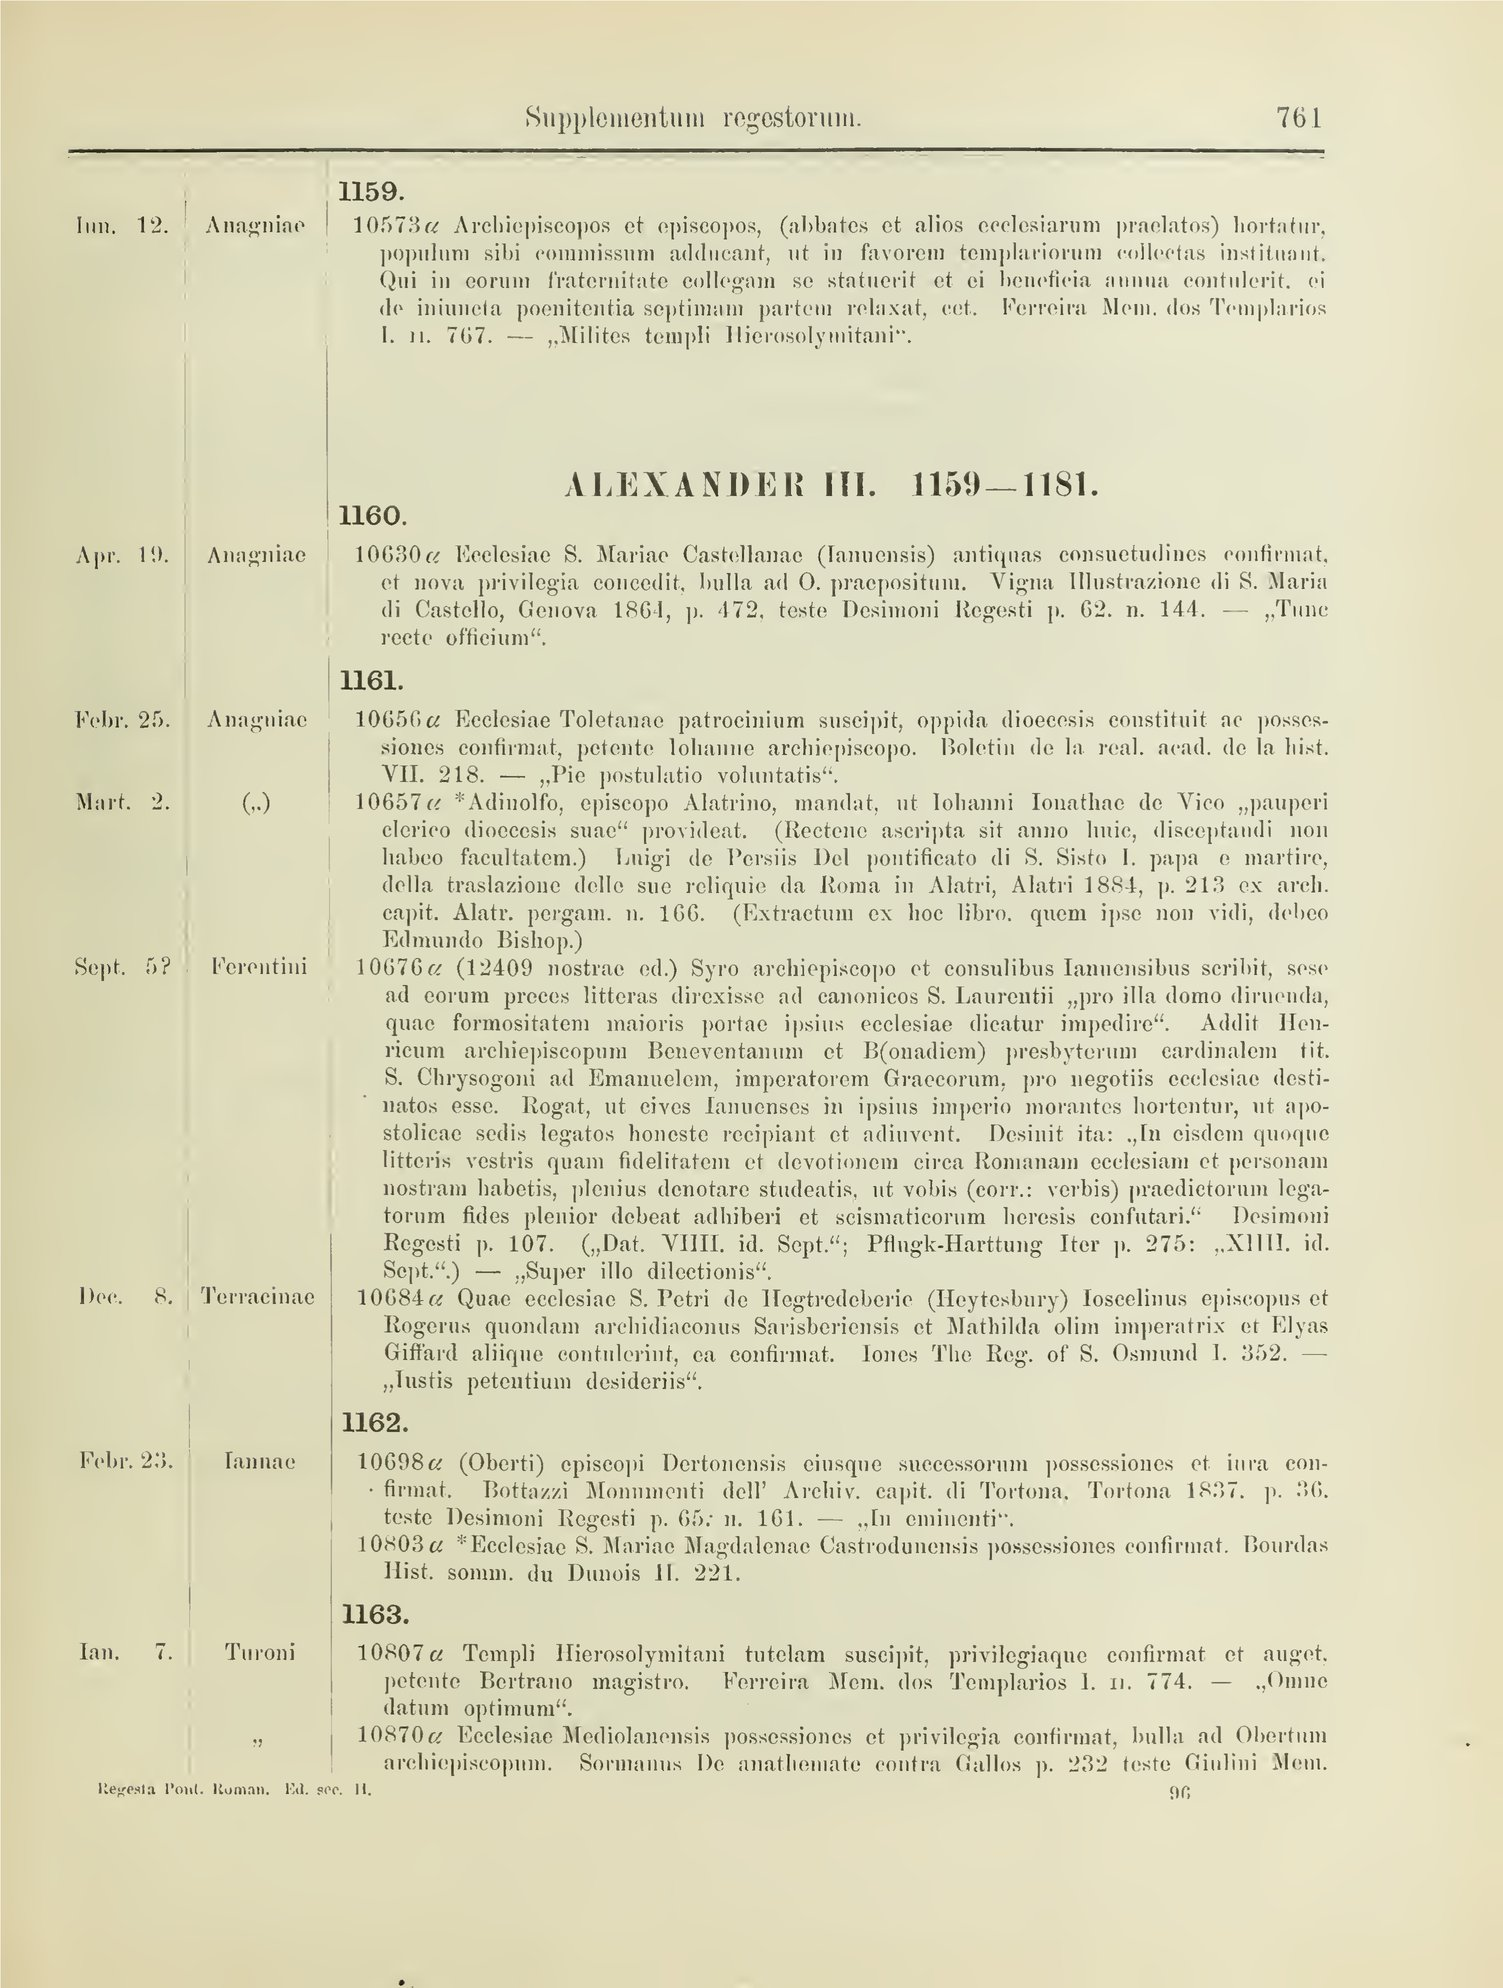
\includegraphics[width=12cm]{images/jaffe2_00772.jpg}
    %légende
    \caption{Exemple d'une page du \textit{Regesta Pontificum Romanorum}, tiré du site du \textit{Monumenta Germaniae Historica} \url{https://www.mgh.de/de}}
    %label
    \label{fig:Jaffe2}
\end{figure}

Le Jaffé permet aux chercheur.se.s de comprendre rapidement le contenu d'une charte, c'est pourquoi c'est une source précieuse pour ce projet.\\

Le schisme alexandrin est la crise la plus importante du XIIème siècle, entraînant une division profonde entre les partisans d'Alexandre III et ceux de l'empire. Néanmoins, la fin de ce schisme s'est accompagnée d'une unification de l'Europe Occidental sous l'égide de l'Eglise.\\ 
On comprend la complexité de ce projet à travers le contexte historique étudié et les différents types de documents et de témoins à intégrer afin de pouvoir potentiellement répondre aux questions que se posent les chercheur.se.s. 
    \chapter{Effectuer un état de l'existant}

Le projet du CCeH compte intégrer l’ensemble des documents ayant trait au schisme alexandrin ainsi que les données des différents projets numériques pouvant témoigner de cette période. Après l’identification des différents acteurs du contexte historique nous intéressant et l’ensemble documentaire à étudier, il est nécessaire de faire un état des projets numériques déjà existants. L’objectif est d’évaluer l’intérêt des données présentées ainsi que les technologies utilisées. Ce travail permet également de réfléchir au modèle de données souhaité. 


    \section{Deux projets de référence}

    \subsection{Le \textit{RI Online}}

Grâce à un projet financé par la \textit{Deutsche Forschungsgemeinschaft}\footnote{Fondation allemande pour la recherche}, les \textit{Regesta Imperii} ont été entièrement numérisés par l’Académie des Sciences et des Lettres de Mayence et la \textit{Bayerische Staatsbibliothek}\footnote{Bibliothèque d’Etat de Bavières.} entre 2001 et 2006 \footnote{Kuczera Andreas, Graphentechnologien in den digitalen Geisteswissenschaften https://kuczera.github.io/Graphentechnologien/ }. Les regesten sont accessibles en ligne sur le site internet RI Online.
Grâce à un portail de recherche, le site permet d’accéder à l’ensemble des 140.000 regesten, stockés dans une base de données MySQL classés principalement par famille puis par empereur. En plus de la consultation des regesten, il est également possible d’accéder aux sources documentaires grâce au RI OPAC, un portail de littérature médiévale en libre accès.
Le RI Online met à disposition les regesten au format HTML ou XML, plus précisément XML-CEI. L’encodage \href{https://www.cei.lmu.de/}{\textit{Charters Encoding Initiative}} (CEI) fut créé en 2004 par un groupe de travail formé à Munich. Ce type de schéma XML est utilisé spécifiquement pour encoder les chartes médiévales. Le RI Online exploite abondamment le standard CEI et est ainsi considéré comme une référence en la matière. Sa plateforme permet notamment d’accéder aux regesten, à la documentation ou à de nombreux liens externes vers d’autres ressources ( par exemple vers le site monasterium.net). Le RI Online dispose aussi d’autres fonctionnalités dont pourrait  s’inspirer le projet du schisme alexandrin. Par exemple, l’IHM (Interface Homme-Machine)  de présentation de documents,  la structure  du schéma CEI, ou  l’API REST permettant la communication des données. 
Certains aspects pourraient néanmoins être améliorés, comme la présentation des descriptions de sources et de la littérature, qui ne sont malheureusement pas structurées, ou les URI vers les fichiers qui sont difficiles d’accès. 


\begin{figure}[h]
%centrer l'image
    \centering
    %commande qui permet de charger une image
    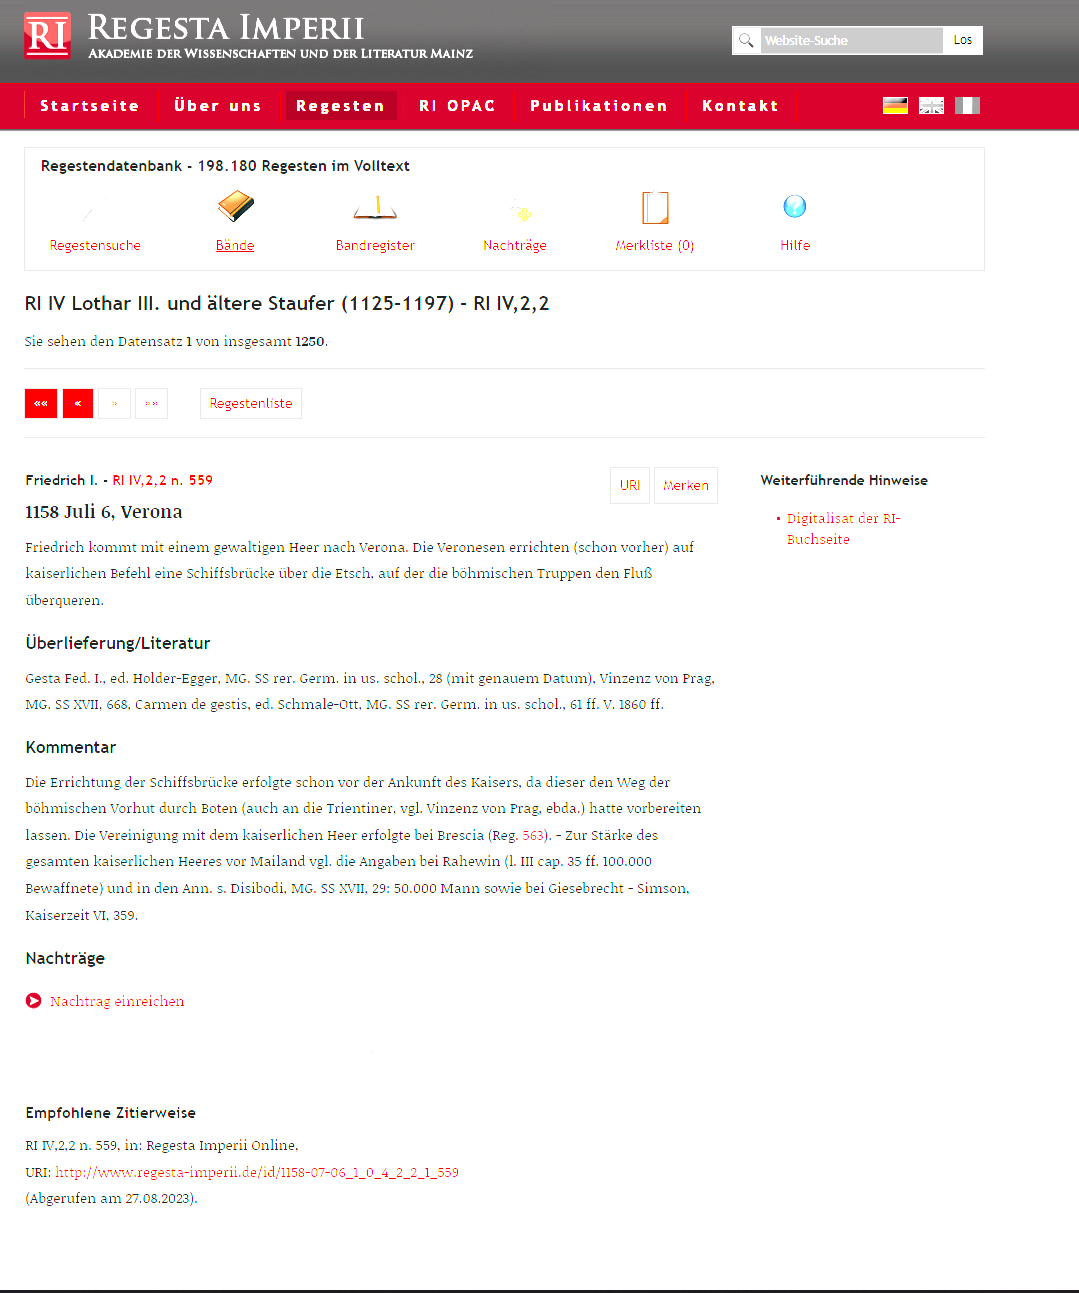
\includegraphics[width=12cm]{images/RI_online.png}
    %légende
    \caption{Capture d'écran du site RI Online, Friedrich I, RI IV,2,2 n. 559}
    %label
    \label{fig:RIonline}
\end{figure}


    \subsection{Le \textit{Papsturkunden}}

Le \textit{papsturkunden} est une collection d'éditions critiques des actes pontificaux jusqu’à Innocent III (1198), menée par la Société des sciences de Göttingen à partir du début du 20ème siècle. Cette édition est composée de répertoires nationaux, le premier étant l'Italia Pontificia entre 1906 et 1975, puis le German Pontificia à partir de 1910, et enfin le Gallia Pontificia sous la direction de l'Institut Historique Allemand (IHA) et l'École Nationale des Chartes\footnote{Hayez, M. (1999), \textit{Gallia pontificia: Répertoire des documents concernant les relations entre la papauté et les églises et monastères en france avant 1198, vol I: Diocèse de Besançon}, par B. de vregille, R. locatelli, G. Moyse et D. lohrmann (book review), Revue d'Histoire Ecclésiastique, 94(3), 927. Retrieved from https://www.proquest.com/scholarly-journals/gallia-pontificia-répertoire-des-documents/docview/1302396270/se-2}. Celui-ci est la suite des travaux de publication du \textit{Papsturkunden in Frankreich}. L'objectif est de réunir sous forme de \textit{regeste} les lettres, actes et autres documents papaux témoignant des contacts entre l’église française et la papauté. 
Entre 2007 et 2022, la Société des Sciences de Gottingen a mené un projet de base de données réunissant les différents répertoires, et en parallèle l'IHA a créé sa plateforme en ligne pour le Gallia Pontificia. Comme pour le RI Online, les bases de données du Papsturkunden et du Gallia Pontificia présentent des avantages qui pourraient être intégrés au projet. Leur principal intérêt est le format de présentation de données, principalement inspiré du Jaffé 2. Par ailleurs, plusieurs liens sont faits entre Jaffé 2 et les documents papaux grâce à l’accès au format PDF du Jaffé et de la cote donnée au document. Jaffé servant de base de référence pour une majorité des documents intégrés au projet, il est nécessaire de toujours proposer le numéro d’entrée du Regesta Pontificum Romanorum. 


\begin{figure}[h]
%centrer l'image
    \centering
    %commande qui permet de charger une image
    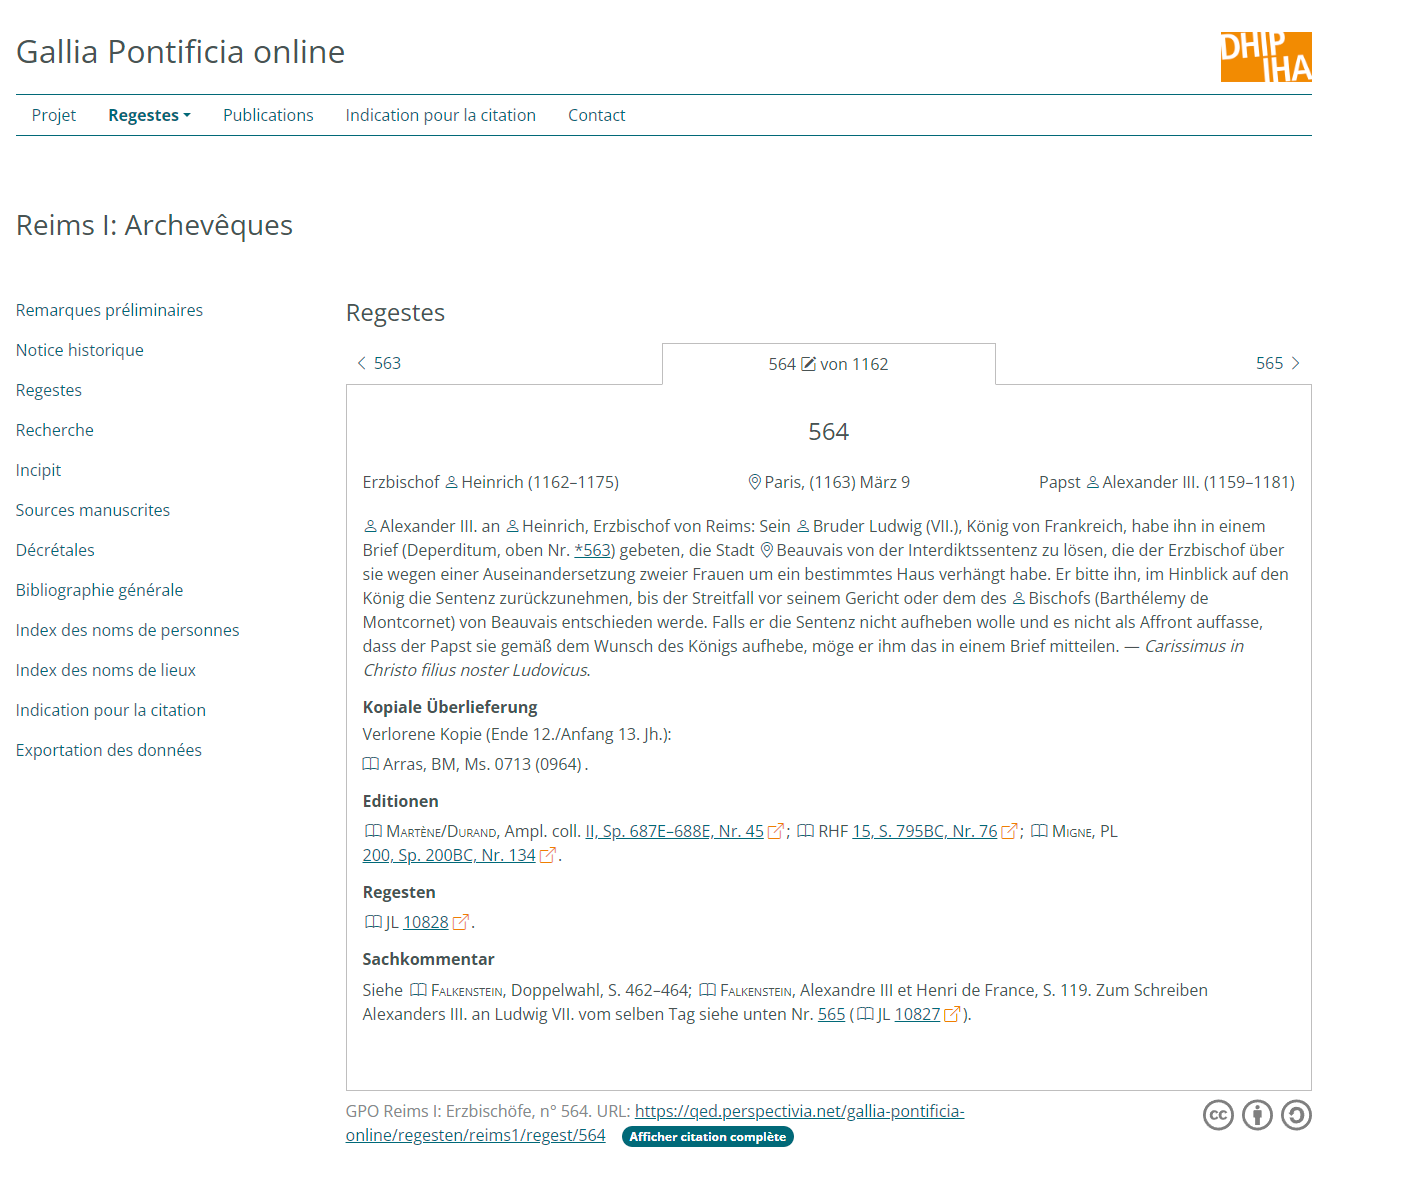
\includegraphics[width=12cm]{images/Gallia_pontificia.png}
    %légende
    \caption{Capture d'écran du site Gallia Pontificia online, regeste n°564}
    %label
    \label{fig:galliapontificia}
\end{figure}


    \section{Des bases de données déjà existantes}

Dans ce travail d’état des lieux des projets existant, on note que les documents papaux sont éparpillés entre plusieurs pays, il est donc nécessaire de s’intéresser à des projets hors du contexte allemand.\\ 
Un des principaux projets les plus intéressants et les plus importants en termes de quantités de données est la base de données française \href{http://telma-chartes.irht.cnrs.fr/}{APOSCRIPTA}, fusionnée récemment avec la base de données Chartae Galliae. Son objectif est de “rassembler les textes et métadonnées du plus grand nombre possible de documents (lettres principalement) émis par les pontifes romains depuis les origines jusqu'à l'âge moderne, quelles que soient leurs traditions manuscrites.” Cette base de données a été lancée en 2017 à l’initiative de plusieurs groupes de recherche, dont \href{https://fulmen.hypotheses.org/category/fulmen-un-programme-de-recherches-collectives}{FULMEN}\footnote{Programme international de recherche qui réunit des historiens de toutes les périodes pour des recherches sur la forme et les usages des censures canoniques de l’Antiquité tardive à nos jours.} et l’université de Lyon II. Elle permet notamment de compléter les données du \textit{papsturkunden} et \textit{Gallia Pontificia}. On compte environ 739 entrées pour le mot clef “Alexandre III”. Les éléments de description du document sont très complets, on retrouve notamment le destinataire, les dates, le lieu, le type de document, l’analyse, parfois la transcription, le numéro Jaffé, la bibliographie.\\

\begin{figure}[h]
%centrer l'image
    \centering
    %commande qui permet de charger une image
    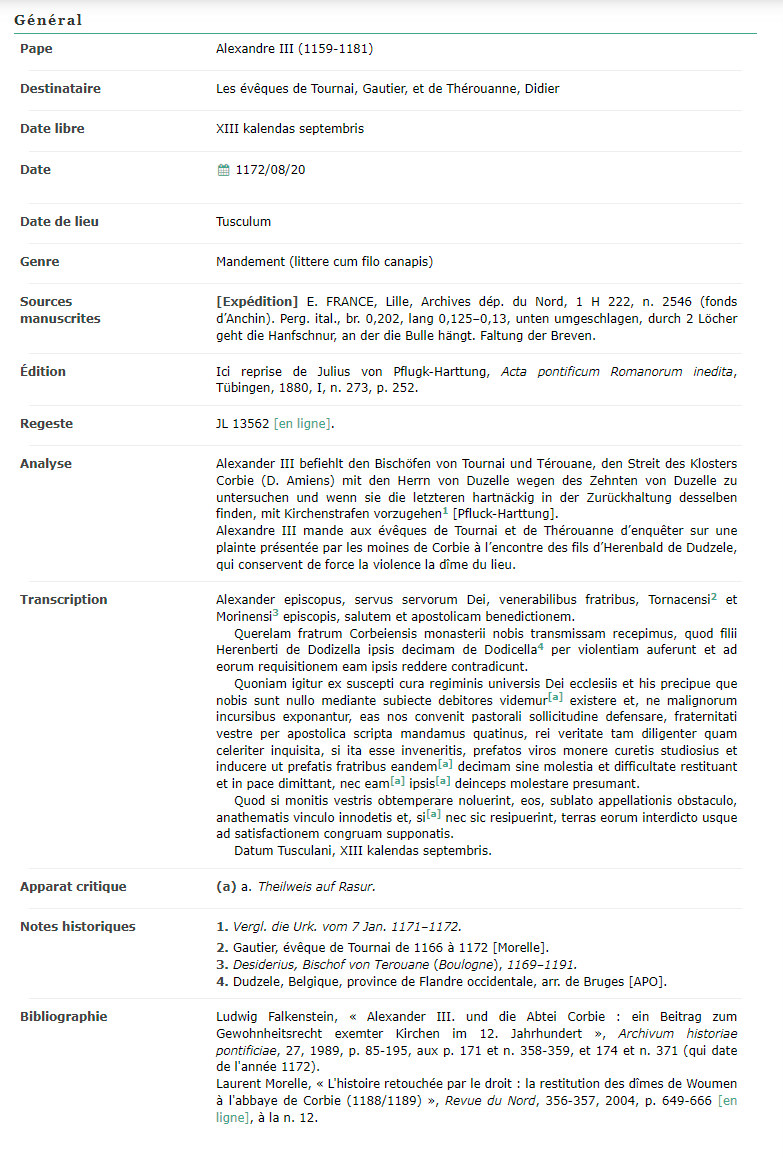
\includegraphics[width=12cm]{images/aposcripta-3461.png}
    %légende
    \caption{Capture d'écran du site APOSCRIPTA, aposcripta-3461}
    %label
    \label{fig:Aposcripta}
\end{figure}


\noindent D'autres projets intéressent les chercheurs du projet du CCeH: 
\begin{itemize}
    \item \href{https://www.diplomata-belgica.be/colophon_fr.html}{Diplomata Belgica}. Initié au milieu des années 1980, ce projet s'appuie sur une base de données réunissant environ 35000 actes expédiés des Pays-Bas méridionaux durant le Moyen-Age. Pour l'entrée "Alexandre III", on compte 483 entrées environ pour Alexandre III. Par ailleurs, le Diplomata Belgica possèdent des bonnes métadonnées et des bonnes fonctions de recherche.
    \item \href{https://deeds.library.utoronto.ca/}{Documents of Early England Data Set} (DEEDS). Ce projet fut initié en 1975 à l'université de Toronto.  inspiration pour la géolocalisation.\\
    
\end{itemize}


Prendre connaissance des données et projets déjà existants -  qui couvrent tout ou une partie du périmètre fonctionnel étudié - est une étape primordiale dans la modélisation de données. L’adoption du projet, la familiarité qu’auront les chercheurs à utiliser l’outil développé dépendra de la bonne intégration des modèles pré-existants dans le modèle conçu.\\
Par exemple, si l’outil développé présentait une lettre pontificale sans faire mention de son numéro Jaffé, le chercheur serait alors bien plus réticent à l’utiliser, pourrait douter de la qualité de l’outil mis entre ses mains, et finirait sans doute par le disqualifier.
C’est pourquoi, une fois l’état des lieux réalisé, il est nécessaire de mettre en place les moyens pour récupérer et intégrer les données existantes dans le projet.



        \chapter{Création, récupération et intégration des données}

Les données sont rarement homogènes ou immobiles\footnote{Les données tendent toujours à évoluer dans le temps, que ce soit par l’ajout de métadonnées par exemple, ou de format etc…} : elles peuvent nous parvenir dans différents formats et sont parfois incomplètes, elles peuvent également s’avérer difficiles à récupérer. Cela met en évidence plusieurs enjeux à examiner :  l’ accès aux données, la pluralité des  formats et la fraîcheur de  ces données (sont-elles complètes, y aura-t-il des mises à jour ?).


    \section{Accès aux données}

La première étape est de pouvoir tout simplement accéder à ces données. En reprenant les exemples des projets mentionnés précédemment, nous allons voir que l’accès aux données peut se révéler moins trivial qu’il n’y paraît.

    \subsection{Du document à la donnée}

Dans un premier temps, il faut considérer la création des données, pour les documents physiques qui ne sont pas accessibles de façon dématérialisées.\\

\noindent \textbf{\textit{Optical Character Recognition}}

L’\textit{Optical Character Recognition} (OCR) est un processus de reconnaissance de caractère d’un texte, ou l’extraction d’un texte d’une image. Il permet de créer des textes numériques à partir de manuscrits exploitables par une machine.\footnote{Schoen Jenna, Saretto Gianmarco E., \textit{Optical Character Recognition (OCR) and Medieval Manuscripts: Reconsidering Transcriptions in the Digital Age}, in \textit{Digital Philology: A Journal of Medieval Cultures}, Volume 11, Number 1, Spring 2022, pp. 174-206.}. L'objectif est de pouvoir facilement chercher et éditer le document numérique.\\
La première étape de ce projet consiste à utiliser l'OCR sur le \textit{Regesta Pontificum Romanorum} afin de faciliter les recherches parmi les entrées.\\

\noindent \textbf{\textit{Handwritting Technical Recognition}}

 Un des moyens possibles de créer de la donnée est la reconnaissance de l’écriture manuscrite (HTR). Une des pistes envisagées dans ce projet est de créer un modèle HTR pour la transcription automatique des chartes mais également pour le Jaffé 2. On peut imaginer que les objectifs seraient dans un premier temps de faire un état de l’art des outils actuels, comme eScriptorium, ayant pour base l’outil Kraken, et Loghi. En effet, différents modèles de reconnaissance de texte existent déjà, donc il est nécessaire de les tester afin d’observer les apports de ces outils déjà existant à ce projet. Il est tout à fait possible de considérer une amélioration de ces outils grâce à leurs entraînements avec le corpus du projet du CCeH comme matériaux. Par ailleurs, si ces outils semblent ne pas convenir suffisamment aux besoins, il est également possible de proposer un nouveau modèle de reconnaissance de texte manuscrits

    
    \subsection{Obtenir une sauvegarde des données}

Certains projets offrent la possibilité de télécharger les données directement sur leur site. RI Online permet de télécharger l’ensemble des quatre volumes en une seule fois sur son site internet. Ce n’est pas le cas de tous les projets. Monasterium.net par exemple ne permet pas de télécharger plusieurs chartes de manière groupée: on ne peut le faire qu’une par une. L’export JSON du projet APOSCRIPTA ne fonctionne pas, il sera ainsi nécessaire de contacter les personnes en charge du projet pour accéder aux données.
L’obtention d’une sauvegarde est une solution convaincante mais incomplète de récupération de données: bien que très simple à mettre en place, elle occulte l’enjeu de la mise à jour des données.  Même si la sauvegarde en question est mise à jour régulièrement, il faut toujours synchroniser deux bases de vérités: la sauvegarde du projet d’origine et les données importées dans votre projet. C’est une solution sub-optimale, coûteuse et sujette aux erreurs; il sera toujours préférable de n’avoir qu’une source de vérité, par exemple, une API.\\

En plus des difficultés d’accès comme ceux ci-dessus, il est possible d’être confronté à un autre problème, celui des projets d’humanités numériques non maintenus. C’est le cas du site du \textit{papsturkunden}, qui est actuellement inaccessible. Il est donc impossible de récupérer une sauvegarde des données directement sur le site internet. Cette absence de maintenance est un enjeu important dans la pérennisation des projets en humanités numériques. Il est difficile de pérenniser un projet dans ce domaine contrairement à des projets dans les entreprises, principalement pour des questions de moyens. Concernant le \textit{papsturkunden}, il fut tout d’abord question de scraper\footnote{Technique d’extraction de données grâce à un script ou un programme.} les données lorsque le site internet était encore accessible. Aujourd’hui, il est envisagé de récupérer le projet au sein du CCeH, mais cela n’est possible que grâce aux relations entre les universités. S’il était question d’un projet français, la démarche de récupération des données serait probablement plus laborieuse.

    
    \subsection{(REST) API}

Une \textit{Application Programming Interface} (API) est une brique logicielle qui permet à deux applications de communiquer entre elles et d’échanger des données. Il existe différents types d’APIs (REST, SOAP, gRPC), qui correspondent à différentes manières de s’échanger des données; nous aborderons ces sujets plus bas . Pour les projets évoqués plus haut ainsi que pour la plupart des projets d’humanités numériques, une API servira essentiellement à partager les données du projet, voire, dans certains cas, à les enrichir. Plutôt que d’intégrer des données d’autres projets en les dupliquant dans votre base de données, vous pourrez désormais envoyer une requête à l’API pour obtenir une donnée fraîche.  
Les API REST (Representational State Transfer) sont les plus populaires car plus simples à développer et consommer que leurs homologues. Elles permettent d’effectuer des opérations CRUD (Create, Read, Update, Delete) sur des données identifiés par une URL via des requêtes HTTP. Prenons l’exemple d’une API qui met à disposition les données du schisme alexandrin à l’adresse https://alexander-project.cceh.de/api. Si les chartes sont identifiés par leur numéro Jaffé, pour récupérer la charte numéro 42, on pourra faire la requête HTTP suivante : 
\begin{lstlisting}
    curl -X GET https://alexander-project.cceh.de/api/charters/42
\end{lstlisting}

\noindent La réponse de la requête contiendra les données relatives à la charte en question. 
Si l’on veut ajouter une charte, cela prendrait la forme suivante : 

\begin{lstlisting}
    curl -X POST https://alexander-project.cceh.de/api/charters
     -H "Content-Type: application/json"
     -d '{"jaffe_id": 4815162342, "transcription": "..."}' 
\end{lstlisting}


\noindent Le RI Online est le seul projet à mettre à disposition une API pour communiquer ses données, il s’agit d’une API REST. Ces bonnes pratiques ne sont malheureusement pas encore très répandues en humanités numériques.


    \section{Formats et transformation des données}

L’autre enjeu de la récupération des données est leur intégration au projet. Il est nécessaire de réfléchir en amont à un modèle de données et au format souhaité. Tout dépendra également de ce que l’on veut faire des données. Nous allons évoquer ici le format XML CEI, adopté pour les fichiers du RI Online.\\ 
Un des objectifs de ce projet est de proposer un nouveau schéma CEI pour améliorer l’ancien qui n’a pas été mis à jour depuis plusieurs années. On commencera par analyser les fichiers XML du RI online afin d’identifier des améliorations possibles. Nous avons réuni les données au sein d’une base de données BaseX. Le choix de la base a été motivé par la familiarité qu’avaient les membres du projet avec cette technologie. 
A partir de l'exemple de fichier XML (annexe \ref{annexe:CEI_schema}) extrait de la base de données réunissant les fichiers XML du RI Online ayant trait à l'empereur Frédéric Ier\footnote{\url{https://github.com/Marine-Tiger/2023_M2TNAH_memoire/tree/main/livrable_technique/RIV_Friedrich1_1122-1190}}, on peut comprendre la nécessité d'avoir un modèle de données bien défini. En effet, en l'état, les fichiers XML semblent peu exploitables si l'on souhaite extraire et étudier certaines informations. On constate que la manière dont sont encodés les noms de personnes rendent difficiles leur extraction. \\ 
Par exemple, pour les témoins présents dans les balises \verb|<testis>|, si on souhaite obtenir une liste, on peut écrire la requête XQuery suivante:\\

\lstset{style=mystyle}
\begin{lstlisting}[language=XML]
<document>
{
for $location in collection("/home/marine/Documents/RIV_Friedrich1_1122-1190/")//issuePlace
return

<place>{$location/placeName[@key]/text() }</place>
}

</document>
\end{lstlisting}

\noindent Voici un extrait du résultat de la requête:\\
\lstset{style=mystyle}
\begin{lstlisting}[language=XML]
<document>
    <witnesses>die Bischöfe Konrad von Worms, Gunther von Speyer, Burchard von Straßburg, Konrad von Augsburg, Dompropst Walter von Köln, Dekan Albert (von Köln), Propst Diepold von Xanten, Abt Nikolaus von Siegburg (), die Pröpste Arnold vom Andreasstift (in Köln), Ulrich von Soest (), die Herzoge Heinrich von Bayern, Heinrich von Sachsen und viele Fürsten; von den Kölner Hintersassen (): Vogt Hermann (von Eppendorf), Heinrich von Volmarstein (), Heinrich von Alpen (), Truchseß Adolf, Schenk Randolf, Raboto von Odenkirchen, Amalrich von Wormersdorf ()</witnesses>
    <witnesses>die Erzbischöfe Humbert von Besançon, Heraclius von Lyon, Petrus von Tarentaise, Bischof Wilhelm () von Novara, Herzog Matthäus von Lothringen, die Grafen Volmar von Saarwerden (), Stephan von Herrlingen (), Albert von Dillingen</witnesses>
    <witnesses>Pfalzgraf Otto von Wittelsbach, Gebhard und Markward von Leuchtenberg und die Brüder Gottfried, Adalbero und Konrad von Salksdorf</witnesses>
    <witnesses>Erzbischof Arnold von Köln, Bischof Ortlieb von Basel, Abt Wibald von Corvey, die Herzoge Heinrich von Sachsen, Welf von Spoleto, die Pfalzgrafen Otto von Wittelsbach, Friedrich von Tubingen ()</witnesses><witnesses>Erzbischof Wichmann von Magdeburg, Bischof Gebhard von Würzburg, die Äbte Markward von Fulda, Adam von Ebrach, Herzog Friedrich von Schwaben, Landgraf Ludwig (von Thüringen), Pfalzgraf Otto der Jüngere von Wittelsbach und sein Bruder Friedrich, die Grafen Gerard von Bergtheim, Poppo von Henneberg () sowie sein Bruder Berthold und Goswin von Tecklenburg (), Markward von Grumbach, Konrad von Pfitzingen (), Giso von Hildenburg (), Sigeboto von Zimmern ()</witnesses>
    <witnesses>die Erzbischöfe Eberhard von Salzburg, Wichmann von Magdeburg, die Bischöfe Hartwig von Regensburg, Eberhard von Bamberg, Konrad von Passau, Otto von Freising (), Daniel von Prag, die Herzoge Heinrich von Österreich, Friedrich von Schwaben, Landgraf Ludwig von Thüringen, die Markgrafen Albrecht (der Bär) von Sachsen, Otto von Meißen, die Pfalzgrafen Otto und Friedrich (von Wittelsbach)</witnesses>
</document>
\end{lstlisting}

Le résultat est plutôt illisible, et si on souhaite extraire les noms pour les mettre dans des fichiers csv (pour étudier l'occurrence des témoins dans une période donnée par exemple), cela paraît difficilement faisable.\\
En comparaison, les lieux dans les balises \verb|<issuePlace>| et \verb|<placeName>| sont bien référencés. On peut par exemple les extraire dans un fichier \verb|csv| grâce à un script python (\ref{annexe:script_python_places}), ce qui permet d'obtenir un jeu de données exploitables par une machine, dont on peut voir l'extrait ci-dessous.\\

\begin{tabular}{|c|c|c|c|c|}
\hline
  \textbf{Date de début} & \textbf{Date de fin} & \textbf{Lieux} & \textbf{latitude} & \textbf{longitude}\\ 
  \hline
  1177-08-22 & 1177-08-22	& im Dogenpalast zu Venedig	& 45.5833 & 12.5667\\
  \hline
  1177-08-01 & 1177-08-31 & Venedig & 45.5833	& 12.5667\\
  \hline
  1169-10-01 & 1169-10-31 & Donauwörth & & \\ 		
  \hline
  1175-01-01 & 1175-12-31 & Rülzheim 	&	& \\
  \hline
  1177-05-10 & 1177-05-10 & Venedig & 45.5833 & 12.5667\\
  \hline
  1178-08-15 & 1178-08-15 & Vienne & 48.2167 & 16.3667\\
  \hline
  1179-06-27 & 1179-06-27 & Burg Kelmünz & & \\
  \hline
  1177-05-11 & 1177-05-11 & Ravenna & 44.4167	 & 11.9833\\
  \hline
  1174-02-24 & 1174-02-24 & auf dem feierlichen & & \\
   \hline
\end{tabular}\newline

Une fois que le nouveau schéma CEI aura été défini, il sera alors possible de convertir les fichiers d’origine vers le nouveau standard à l’aide de XSLT, une technologie dédiée à la transformation de documents XML. 


    \section{Mise à jour de la donnée}

Comme évoqué auparavant, la complexité de l’actualisation des données dépendra des moyens mis en œuvre pour récupérer lesdites données. En prenant l'exemple des données du RI Online, on peut imaginer trois scénarios concernant la mise à jour des données en fonction de la récupération. 

    \subsection{Cas de sauvegarde des données}

Si nous récupérons les données en les téléchargeant, cela permet de conserver les données au sein du projet du CCeH, et d'accéder à l'ensemble des données, ce qui n'est pas possible lorsque l'on accède aux données grâce à une API.
Afin de mettre à jour les données, il est nécessaire d'écrire un script de synchronisation des données. Cela permet de faire correspondre les informations stockées dans des endroits différents. L'inconvénient dans ce cas de figure est qu'il y a un risque d'avoir deux vérités, puisque le RI Online peut effectuer des modifications dans sa base de données sans que l'on puisse les récupérer en temps réel.\\ 

\begin{figure}[H]
%centrer l'image
    \centering
    %commande qui permet de charger une image
    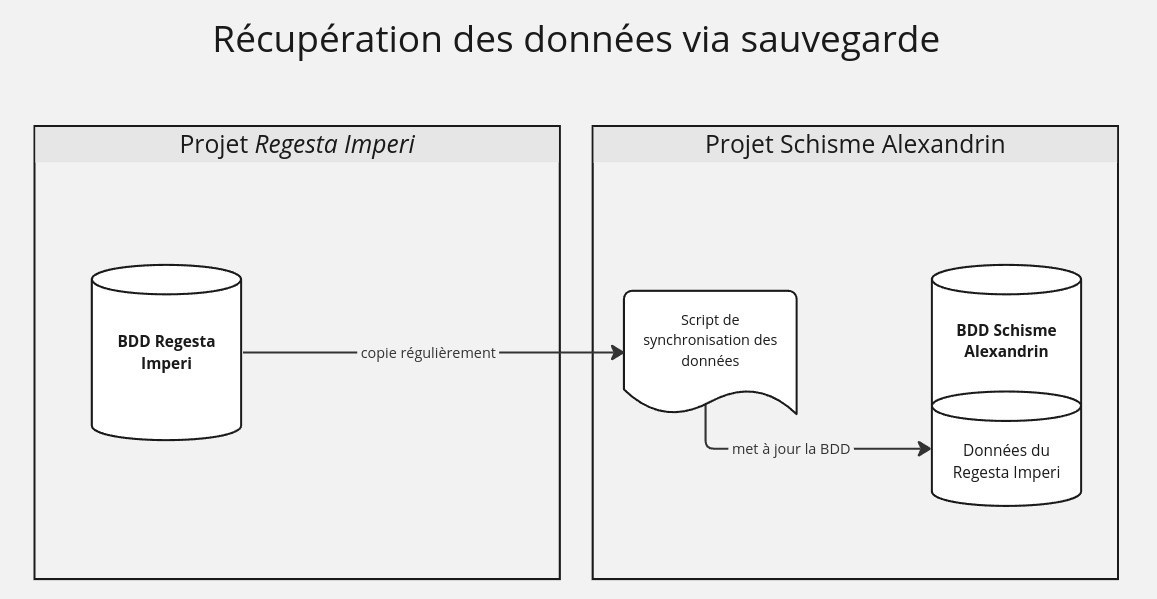
\includegraphics[width=10cm]{images/recup-donnees-sauvegarde.jpg}
    %légende
    \caption{Schéma représentant la récupération des données manuellement}
    %label
    \label{fig:schemadonneessauvegarde}
\end{figure}


    \subsection{Cas des données récupérées grâce à une API}

En récupérant les donnés à partir d'une API, nous nous assurons de toujours récupéré les données à jour. Par ailleurs, cette solution est plus facile car il est juste nécessaire de se connecter à l'API du projet. Mais le risque repose sur le fait que si le projet est abandonné ou plus maintenu, nous risquons de ne plus accéder aux données car l'API ne fonctionnera plus également.\\

\begin{figure}[H]
%centrer l'image
    \centering
    %commande qui permet de charger une image
    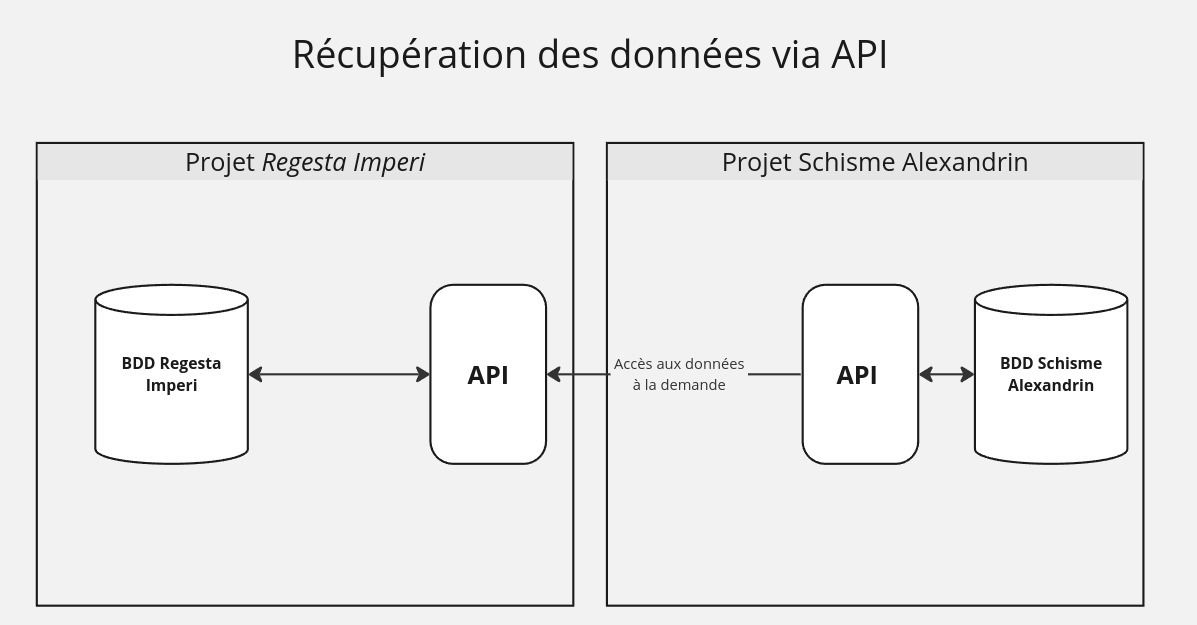
\includegraphics[width=10cm]{images/recup-donnees-api.jpg}
    %légende
    \caption{Schéma représentant la récupération des données grâce à une API}
    %label
    \label{fig:schemaAPI}
\end{figure}

    \subsection{Cas des données récupérées grâce à une API et une sauvegarde des données}

Ce dernier cas de figure présente une solution idéale, puisqu'elle consiste à récupérer les données à la fois grâce à l'API et en téléchargeant les données. Cela permet de s'assurer d'avoir toujours accès aux données à jour en ayant à la fois une connexion à l'API et un script de synchronisation de données. Par ailleurs, si le RI Online n'est plus maintenu, on est assuré d'avoir les données au sein du projet. En revanche, cette solution est plutôt coûteuse à mettre en place et à maintenir.\\

\begin{figure}[H]
%centrer l'image
    \centering
    %commande qui permet de charger une image
    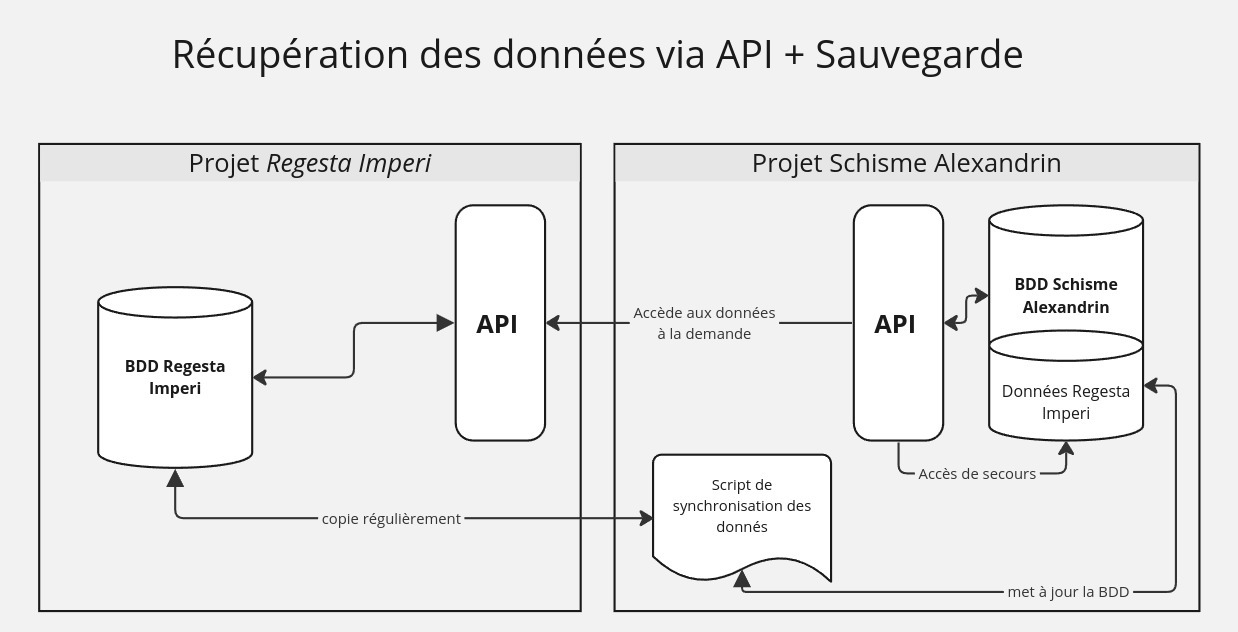
\includegraphics[width=10cm]{images/recup-donnees-api-and-backup.jpg}
    %légende
    \caption{Schéma représentant la récupération des données manuellement et grâce à une API}
    %label
    \label{fig:schemaAPIetbackup}
\end{figure}





La modélisation de données a permis de mettre en lumière plusieurs enjeux concernant le projet du schisme Alexandrin. Tout d’abord, le contexte historique dépeint de nombreux faits et acteurs rassemblés dans un corpus documentaire très vaste, estimé à environ 11.000 documents à terme. Ensuite, l’analyse de divers projets d’humanités numériques nous a permis d’évaluer les modèles de données et technologies à envisager. Les chercheurs de Aachen veulent s’inspirer des entrées du papsturkunden et du Regesta Pontificum Romanorum, et utiliser le schéma XML CEI. Enfin, s’atteler à la récupération de ces données peut s'avérer complexe :  celles-ci sont éparpillées entre plusieurs projets, sous différents formats et accessibles de manière non-uniforme. Actuellement, le premier objectif de ce projet est d’accéder au Jaffé 2 grâce à l’OCR, afin de pouvoir faciliter la recherche textuelle, et à terme pouvoir le traduire en anglais. Il est également important de noter que pour le moment, seulement les données du RI Online sont accessibles, et seraient ainsi les premières à être intégrées au projet.
	
	\part{Enjeux des choix technologiques, ou le \textit{system modeling}}
    
    Le \textit{system modeling} ou \textit{software modeling} correspond à la modélisation des briques logicielles qui feront le projet, il s’organise autour d’une réflexion des besoins, déjà évalués lors de la modélisation de données. 
Le projet sur la formation de l’Europe au 12ème siècle est confronté à un enjeu de durée s'étend sur 18 ans, période durant laquelle de nombreuses technologies apparaîtront et disparaîtront. Il s’agit d’une problématique commune à tous les projets envisagés sur le  long terme: quelles technologies utiliser?  Devons-nous tester, expérimenter avec les nouvelles technologies, les nouveaux logiciels et langages de programmation? \\
Il est nécessaire de rappeler que nous sommes à la genèse du projet sur le schisme alexandrin, les pistes évoquées ici sont hypothétiques. En revanche, l’objectif est aussi de tendre vers une réflexion plus vaste autour des attentes d’un projet long en humanités numériques. Pour aider dans cette réflexion, nous avons effectué des réunions avec les différents ingénieurs du CCeH pour qu’ils nous introduisent aux différents projets en cours. Cela permettra d’analyser les forces et les faiblesses des technologies déjà utilisées au sein du CCeH.


    
    \chapter{Réunir les données}

Nous avons pu établir précédemment que les différents corpus documentaires sont pour la plupart déjà accessibles de manière dématérialisée, mais dispersés entre les différents projets d’humanités numériques. Le premier objectif, une fois le modèle de données établi, est donc de réfléchir à la manière dont nous souhaitons conserver ces données. Ainsi s’ouvre la réflexion à propos du choix de la base de données. 

    \section{Types de bases de données envisagées}

    \subsection{Le choix habituel en humanités numériques: base de données document}

Les données concernées sont pour une majorité d’entre elles au format XML. Le format XML est considéré comme un langage très pérenne\footnote{Pierazzo Elena, \textit{Textual Scholarship and Text Encoding}, in Schreibman Susan, Siemens Ray et Unsworth John, \textit{A new companion to Digital Humanities}, Wiley Blackwell, 2016, p307-321.}, et apparaît comme le choix le plus évident dans un projet d’humanités numériques comme celui-ci. Il est nécessaire dans ce cas d’utiliser une base de données de type document, qui permet de gérer des fichiers au format XML. Il y a deux grandes bases de données pour stocker nos données, chacunes ayant ses avantages et ses inconvénients:\\

\begin{itemize}
    \item eXist DB, qui est plutôt simple d’utilisation, permet de rapidement travailler sur les données et d’utiliser les frameworks XRX\footnote{Un framework correspond à un ensemble de logiciels et qui aide à utiliser du code mais qui impose un cadre précis dans le développement du frontend (partie visible pour les utilisateurs) et/ou le backend. En opposition, les librairies permettent également d’utiliser un ensemble de logiciels mais sans cadre imposé. Le framework XRX utilise Xforms (formulaire créé en XML), Rest et XQuery.}
    \item BaseX, qui permet de gérer une quantité importante de fichiers, et possibilité de connecter la base de données grâce à une API Rest.\\
    
\end{itemize}

\noindent Une base de données orientée document est un choix intéressant si le projet se concentre principalement sur la structure du document et à l’information qu’il contient. Elle permet de faire des recherches grâce aux balises. En revanche, plusieurs limites apparaissent en utilisant ce type de base de données:\\ 

\begin{itemize}
    \item être très vigilant sur la normalisation des noms de personnes et de lieux afin d’éviter les doublons. Cela vaut également si l’on veut ajouter des noms grâce à un formulaire par exemple. Il est possible d’éviter les erreurs grâce aux attributs, mais cela signifie prendre du temps pour vérifier que les attributs soient entrés correctement
    \item difficile de représenter des relations entre les personnes (liens familiaux par exemple) ou entre les personnes et les lieux. C’est bien évidemment possible, mais c’est un travail fastidieux qui demande de créer un fichier séparé pour l’ensemble des relations, qui apparaissent dans les attributs.
    
\end{itemize}

    
    \subsection{Les bases de données relationnelles}

Les bases de données relationnelles peuvent être une alternative aux bases de données document. Apparues dans les années 1980, les données y sont organisées en tables distinctes sans niveau de hiérarchie. Elles permettent de représenter les relations entre les différentes entités. Certaines bases de données relationnelles permettent de stocker des documents. On pense par exemple à PostgreSQL, qui offre un bon support du format JSON, avec de bonnes  performances à la clef. Pour un projet comme celui du CCeH, où le volume de données est assez faible comparé aux volumes que peuvent traiter les entreprises privées, stocker les documents dans une base relationnelle pour mieux tirer parti des autres avantages qu’offrent celles-ci est envisageable.\\ 
Un des avantages majeur à choisir une base de données relationnelle est de pouvoir exploiter des contraintes. Il s’agit de règles de maintien  de l’intégrité référentielle, une fois que vous définissez une règle, votre base de données vous empêchera de la violer en refusant les modifications qui contreviendraient à la règle. Cela vous permettra par exemple de définir les contraintes suivantes :\\
\begin{itemize}
    \item Chaque personne enregistrée en base de donnée ne doit l’être qu’une fois, il pourrait cependant avoir différents alias
    \item Les dates de naissances d’une personne doivent être définies de telle sorte que nul ne peut vivre plus de 130 ans
    \item La date d’édition d’une charte par un auteur doit être comprise entre son année de naissance et de décès
    \item Une personne ne peut pas voyager à plus de 60km/h. Formulé autrement, s’il est mention d’une même personne à deux points séparés d’une distance d et d’une durée t, alors d/t < 60.\\
    
\end{itemize}

\noindent Plus les contraintes sont précises et capturent la réalité du monde dans lequel s’inscrivent les données, plus vous serez capables d’identifier des incohérences dans vos jeux de données.\\
Autre avantage non négligeable des bases relationnelles : les relations elles-mêmes. Bien qu’il soit possible d’émuler un système relationnel dans une base documents, cela reste bien moins puissant que ce qu’ont à offrir les bases relationnelles et bien plus complexe à mettre en œuvre et maintenir.
Avec une extension pour la gestion des données géospatiales (PostGIS pour PostgreSQL par exemple), on peut imaginer la fonctionnalité suivante : requêter la base pour obtenir les tracés en GeoJSON des pays/régions administrés par des souverains soutenant Alexandre III chaque année de 1159 à 1181. Ces données permettraient de construire une carte intéractive des nations soutenant Alexandre III au cours de son exercice.


    
    \subsection{De nouvelles perspectives? Les bases de données graphe}


Une base de données orientée graph est un modèle où la structure des données est représentée sous forme d’un graphe\footnote{Angles Renzo, Gutierrez Claudio, \textit{Survey of graph database models}, 2008, 39 pages, p5, https://doi.org/10.1145/1322432.1322433.}. Elle peut être utilisée s’il est envisagé de considérer les relations et les informations tout aussi importantes. Une base de données graphe représente le texte comme une sorte de réseau où il est possible de naviguer grâce aux nœuds dans le texte. Si on prend le format XML TEI ou CEI, les nœuds correspondent aux balises.

Exemple issu du Regesta Imperii de Frédéric III

→ présente une bonne visualisation de données. Alternative du XML?
→ problème: principalement  Neo4j comme base de données. Pour un projet aussi long, peut-être pas le plus sûr. Mais comme 18 ans de projet, peut être envisagé faire des tests.


    \section{Une base de données unique?}

Cette question peut paraître étonnante. En effet, dans beaucoup de projets comme celui-ci, il est courant d’utiliser une seule base de données, mais, en termes de durabilité et d’objectifs du projet, il faut questionner l’usage de différents types de bases pour répondre aux différents enjeux introduits par nos données. 


    \subsection{Avantages}

Il paraît beaucoup plus intuitif de stocker nos données au sein d'une même base. C’est humainement plus facile, car il n’y a qu’un seul langage de base de données à connaître, une seule connexion entre notre application et la base à gérer et enfin une seule base à maintenir  En effet, si on multiplie les moyens de stockage, on multiplie alors aussi les opérations de maintenance, les vulnérabilités potentielles, l’effort requis pour répliquer le projet, les sauvegardes et les compétences nécessaires à la compréhension du projet. 
Par ailleurs, l’ajout d’une nouvelle base de données implique la gestion de la dépendance entre les données des deux bases. À l’instar d’une base de données relationnelle qui garantit l’intégrité référentielle entre les données de différentes tables, il nous faudra gérer l’interopérabilité des données de nos deux bases.\\
Néanmoins, s’astreindre à n’utiliser qu’une seule base de données - et donc une seule manière de représenter nos données - a aussi des inconvénients.
    
    \subsection{Inconvénients}

Si vos données revêtent plusieurs formes, comme c’est le cas pour le projet du schisme Alexandrin, vous vous retrouverez rapidement, comme un nourrisson, à tenter de faire rentrer un carré dans un cercle. Choisissez une base XML et vous 
format unique (pas toujours adapté à une multitude de type de données); contraintes techniques imposées par le type de base choisi. Comme vu précédemment, si choisi base de données XML, la partie relationnelle est complexe, plus facile d’envisager une deuxième base de données pour la partie relationnelle.\\ 
Dans le secteur privé, il est très courant de voir des projets utiliser plus d’une base de données. Chaque base répond à un besoin bien spécifique, qui fait qu’elle sera favorisée par rapport à une autre. Par exemple, si vous avez besoin de mettre en place un cache pour accélérer votre application, il ne sera pas rare d’ajouter une base Redis à votre projet. Si vous voulez ajouter une fonctionnalité de recherche avancée à votre application, vous vous tournerez alors vers ElasticSearch. Ne soyez alors pas surpris de découvrir des projets avec plus de 3 types de bases différentes qui coexistent, c’est une pratique très commune. 

        \chapter{Exploitation (future) de la donnée}

En plus de réfléchir à la ou les bases de données à utiliser, il est également nécessaire de penser à l’utilisation future de la donnée. En effet, il convient de choisir les outils et les interfaces de façon à pouvoir répondre aux besoins des utilisateurs. Dans le cadre du projet sur la formation de l’Europe au XIIème siècle, la future plateforme a pour vocation d’être utilisée spécifiquement dans le cadre de la recherche. Le public visé se compose donc principalement de chercheurs et étudiants. L’enjeu ici est de pouvoir répondre à des questions de recherche.



    \section{Durabilité des technologies}

Nous avons déjà évoqué la question de la durabilité des technologies lors de la présentation des différents types de bases de données. C’est un enjeu important dans le choix des technologies, notamment pour des projets s’étirant sur plusieurs années comme celui du schisme alexandrin.
En effet, certaines technologies peuvent être abandonnées à un temps donné. Pour illustrer ce propos, nous examinerons trois exemples de technologies devenues impopulaires voire obsolètes: un logiciel, un langage et un format de données.

    \subsection{Adobe Flash Player}
    
Flash Player était un logiciel permettant de visualiser du contenu multimédia ( vidéos, images) sur un navigateur web. Fin 2017, Adobe annonce que Flash ne sera plus maintenu, puis fin 2020, Flash est totalement déprécié\footnote{Terme utilisé en programmation, indique qu'un système n'est plus utilisé ou a été remplacé par quelque chose de plus moderne} et n’est plus supporté par l’ensemble des navigateurs web.
La plateforme Flash était utilisée dans différents domaines, comme par exemple dans des services d’archives ou encore en littérature électronique\footnote{Oeuvre littéraire nativement numérique et supposée être lu par un ordinateur. Heckman David, O’Sullivan James, \textit{Electronic Literature: Contexts and Poetics} in \textit{Literary Studies in the Digital Age}, 2018, \url{https://dlsanthology.mla.hcommons.org/electronic-literature-contexts-and-poetics/.}}. Dans ce dernier cas, Flash Player permettait aux auteur.rice.s d’expérimenter avec des outils de créations\footnote{Salter Anastasia, Murray John, \textit{E-Lit after Flash: The Rise (and Fall) of a “Universal” Language}, in Grigar, Dene et O’Sullivan James \textit{Electronic Litterature as Digital Humanities: contexts, forms and pratices}, BloomsBury Academic, 2021, p267-274}. 


    \subsection{Ruby}

Ruby est un langage de programmation orienté objet créé durant les années 1990. Il connut un succès conséquent pendant quelques années, notamment car le langage  est considéré plus flexible que ses concurrents et qu’il permet d’augmenter la productivité des développeurs. Ruby est essentiellement utilisé pour du développement web, notamment avec  son framework le plus populaire: Ruby on Rails (RoR). Ruby est utilisé dans plusieurs projets d’humanités numériques, comme le Deutsche Inschriften au CCeH par exemple.
Ruby est un langage qui perd de plus en plus d’intérêt auprès des développeurs, à cause de son écosystème complexe, de ses faibles performances et de la concurrence rude d'autres langages (Node.JS, Python). 
Comme on peut le constater dans les diagrammes en annexe(\ref{annexe:Ruby_stats}), Ruby est un langage assez peu utilisé, il apparaît même 16ème parmi les langages utilisés par les sondé.e.s en 2023. Par ailleurs, on constate que les utilisateur.rice.s préfèrent Node JS ou encore Python à Ruby. 


    
    \subsection{JPEG2000}

Le JPEG 2000 est un format présenté en 2000 qui permet notamment de compresser une image sans perdre en qualité, il est très utilisé en archives ou en bibliothèques. Par exemple, la Bibliothèque Nationale de France (BnF) a remplacé progressivement le format TIFF par le JPEG2000 depuis 2015\footnote{Cavalié Etienne, Caron Bertrand, \textit{Formats de données pour la préservation à long terme : la politique de la BnF}, version 3 du 9 septembre 2021, pages 81, p46.}. Ce dernier est maintenant utilisé comme format de référence pour la numérisation des plans à la BnF\footnote{\textit{Ibid}.}.\\
Aujourd’hui, plusieurs questions se posent: JPEG2000 n’est supporté que par très peu de navigateurs, a des soucis pour s’adapter à l'Open Source et est un format assez complexe\footnote{\textit{Lack of performant open source decoding software}, Open Preservation Foundation, https://wiki.opf-labs.org/display/TR/Lack+of+performant+open+source+decoding+software }. Beaucoup considèrent ce format comme une technologie de niche, difficile à implémenter. L’intégrer dans un nouveau projet pourrait s’avérer risqué.\\

Ces trois exemples nous permettent de saisir l’importance de l’évaluation de la durabilité des technologies considérées pour notre projet. Pour ce faire, les axes suivants sont à envisager:\\

\begin{itemize}
    \item Utiliser des logiciels Open Source, car il est plus probable qu’ils soient maintenues sur le long terme, voire repris par la communauté. De plus, cela permet de réduire le coût du projet.
    \item Estimer la pérennité d’une technologie en fonction de la taille de sa communauté. Par exemple, le XML TEI est une grande communauté, notamment avec les \textit{guidelines} et le TEI consortium, ce qui en fait, comme dit plus haut, un langage pérenne et un choix sûr. De la même manière, le SQL existe depuis près de 50 ans.\\
    
\end{itemize}


Le choix des technologies à utiliser dans un projet devient très vite un casse-tête, car il faut pouvoir à la fois choisir des logiciels et des langages accessibles aux chercheurs qui n’ont pas spécialement de formation en informatique tout en répondant aux besoins très spécifiques du projet.


    \section{Faire le lien entre les chercheur.se.s et la donnée: UX/UI}

L’user experience (UX) est défini dans la norme ISO 9241-110:2010 comme les perceptions et réponses d’un individu découlant de l’utilisation et/ou la future utilisation d’un produit, d’un système ou d’un service\footnote{Allam, Hussin, Dahlan, \textit{User Experience: Challenges and Opportunities}.}. L’objectif est de prendre en compte les besoins des utilisateurs, ici principalement les chercheur.se.s tout en proposant une interface ergonomique. L’user interface (UI) correspond à la façon dont l’utilisateur visualise les données. \\
L’intérêt de s’intéresser à ces deux notions réside dans la volonté de faire adopter le projet et la plateforme par les utilisateurs. 
    
    \subsection{Interfaces graphiques}

L’interface graphique est un élément crucial du projet, sa qualité et sa facilité d’utilisation doit être une préoccupation majeure car une plateforme qui ne convient pas à l'utilisateur devient rapidement une plateforme inutilisée.\\ 

Dans le secteur privé, c’est l’UX/UI Designer qui se charge de la conception visuelle du produit. Il a pour mission de comprendre les besoins des utilisateurs et d’imaginer l’interface la plus claire pour répondre à ses besoins.
En humanités numériques, comme dans d’autres secteurs où les moyens financiers sont moins importants, cette responsabilité revient généralement au développeur. Cependant, celui-ci ne pourra être aussi compétent qu’une personne dont c’est le métier. Ainsi, lorsque c’est possible, allouer des fonds pour recourir à un expert du design paraît sensé.\\  
Le choix des technologies utilisées pour développer l’interface graphique n’aura pas d’impact sur l’interface elle-même, mais influera sur la simplicité de son développement et sur sa maintenabilité. Par ailleurs, sur un projet de 18 ans comme celui du CCeH, il est important d’envisager que la plateforme va évoluer, que ce soit à la demande des utilisateurs pour une amélioration de l’interface, ou pour l’ajout de fonctionnalités qui toucheront à l’interface. Les langages de base pour le développement d’interfaces web sont bien connus : \verb|HTML/CSS/JavaScript|, mais de nos jours, avec la complexification des interfaces à développer, c’est le choix des frameworks et librairies associés à ces langages qui importe le plus. Au CCeH, \verb|VueJS| semble être le framework \verb|JavaScript| le plus populaire. D’autres alternatives existent, comme par exemple \verb|React| ou \verb|Angular|. Chaque framework ou librairie apporte son lot d’avantages et inconvénients, le choix de l’un plutôt que l'autre dépend essentiellement de la familiarité des développeurs avec celui-ci. Néanmoins, certaines fonctionnalités peuvent faire pencher la balance. Par exemple,  laisse moins de latitude au développeur et offre une expérience de développement bien plus cadrée que \verb|VueJS| ou \verb|React|, ce qui peut constituer un avantage important dans un projet d’humanités numériques où les développeurs ne viennent que rarement du monde de l’informatique. Par ailleurs, en ce qui concerne les mises à jour, \verb|Angular| intègre des outils qui permettent de faciliter la montée de version en modifiant automatiquement le code, diminuant ainsi le coût de maintenance. \\ 
Il est également envisagé de donner un accès aux utilisateurs à la plateforme en s’inspirant du modèle du projet \href{https://www.itineranova.be/in/home}{Itinera Nova}. Initié en 2009 par les archives municipales du Louvain et développé par le CCeH, ce projet a pour objectif de numériser et mettre à disposition l’ensemble des registres des juges et les livres comptables de la ville de 1361 à 1795. Itinera Nova utilise actuellement un framework XRX, évoqué plus haut, et permet de gérer plusieurs niveaux d’accès à la plateforme. En effet, les transcriptions des documents d’archives se font par un groupe de volontaires, qui ont un compte utilisateur, puis sont vérifiées et validées par des administrateurs. Des réflexions autour de la mise en place d’un système de droits doivent donc être engagées.


    \subsection{Formats de données}


Ces dernières années, le JSON s’est imposé comme format de données principal pour le développement d’APIs. Il est simple à lire et à traiter informatiquement. Toutefois, il peine à trouver sa place dans le domaine des humanités numériques où le XML semble lui être préféré. Cela n’est pas un hasard, car même s’il est possible de représenter en JSON des graphes acycliques (arbres) comme le fait le XML, le résultat devient illisible pour un humain. Ainsi, certaines données sont mieux représentées en JSON et d’autres en XML. Par exemple, il conviendra d’utiliser le XML pour une édition numérique de charte, alors que le JSON serait préférable pour lister l’ensemble des lieux visités par un pape.\\
Pour autant, la plupart des APIs ne proposent qu’un format de données, mais ce n’est pas une fatalité: le protocole HTTP prévoit qu’un serveur puisse communiquer avec différents formats de données. L’en-tête HTTP Accept permet d’indiquer au serveur le format auquel on souhaite recevoir la donnée (par exemple : “Accept: application/json” ou “Accept: text/xml”). Plusieurs choix s’offrent alors à nous :\\
\begin{itemize} 
\item Se contenter d’un seul format de données, par manque de moyens ou de temps
\item Proposer l’ensemble de l’API développée aux formats JSON et XML, le client configurera sa préférence grâce à l’en-tête HTTP Accept
\item Segmenter les entités représentées par l’API selon qu’elles soient mieux représentées en JSON ou en XML et ne proposer qu’un seul format de retour par route d’API. On aurait ainsi les éditions numériques en XML et les données spatiales en JSON.
\end{itemize}

    
    \section{Favoriser la collaboration et l'échange}

 Le projet du schisme alexandrin devrait se matérialiser au travers d’une plateforme internationale et collaborative. Afin de garantir une interopérabilité, une connectivité et une utilisation durables des données,  nous appliquerons les principes FAIR: \textit{Findable, Accessible, Interoperable, and Re-usable}. Ces principes sont issus du mouvement de l’\textit{open science}, dont l’objectif est de permettre la réutilisabilité des données générées au cours des projets de recherche\footnote{Francesco Beretta, \textit{A challenge for historical research: Making data FAIR using a collaborative ontology management environment (OntoME)}, in \textit{Semantic Web}, 2021, p279-294.}.
Les principes FAIR sont utilisés afin de guider la production et la publication des données issues de la recherche\footnote{Beretta Francesco, \textit{Données ouvertes liées et recherche historique : un changement de paradigme}, 2023, \url{https://journals.openedition.org/revuehn/3349}}. \\
Une partie de ces principes ont finalement déjà été évoqué précédemment: \\
\begin{itemize}
\item \textit{Findable}: les données doivent avoir un identifiant unique et persistant, décrites avec des métadonnées riches, et indexées. Cette étape se retrouve dans la modélisation des données et dans le modèle de données.
\item \textit{Accessible}: les données doivent être récupérables par leur identifiant à l’aide d’un protocole standardisé et gratuit. Les métadonnées doivent être accessibles même si la donnée n’est plus disponible. Les APIs REST utilisent le protocole HTTP.\\
\end{itemize}

Dans le cadre de la collaboration et des échanges, les principes d'interopérabilité et de réutilisation des données sont primordiaux.



    \subsection{Interopérabilité}

L’interopérabilité doit faire partie des réflexions menées dans les choix technologiques pour les projets d’humanités numériques. Selon les principes FAIR, l’interopérabilité se caractérise de la façon suivante:\\
\begin{itemize} 
\item un langage qui permet la compréhension commune des objets numériques
\item des références à des données externes\\
\end{itemize}
Dans le cadre du projet du schisme alexandrin, il est prévu  de permettre l’export des données au format RDF: un des langages préconisés par les principes FAIR. 
Il sera aussi possible d’accéder à la littérature du RI OPAC ainsi qu’à des liens vers le \href{https://viaf.org/}{VIAF}, le fichier d’autorité international virtuel.\\
De manière plus globale, la norme ISO/CEI 2382-18 définit l’interopérabilité comme étant l’aptitude de plusieurs unités fonctionnelles à coopérer pour traiter des données. Ainsi, choisir des protocoles de communication et des formats de données répandus et simples à implémenter permettra d’augmenter l’interopérabilité du système développé. Par exemple, le protocole SOAP - qui impose le XML comme format d’échange et est considéré complexe à implémenter - ne devait être le premier choix de quiconque souhaitant développer un système interopérable. Il faudra favoriser le REST, plus simple à implémenter et qui ne restreint pas l’usage d’un format de données spécifique.\\
La présence et même le format d’une documentation influe également sur l’interopérabilité du projet réalisé. En effet, impossible d’implémenter une API non documentée ou de tirer pleinement parti d’un outil non documenté. L’édition d’une documentation d’API à un format standardisé (OpenAPI) favorisera ainsi l’adoption du projet développé. Il est préférable, lorsqu’on implémente une API, de visualiser une documentation OpenAPI grâce à l’éditeur Swagger (editor.swagger.io) plutôt que de consulter une documentation au format PDF.

    \subsection{Réutiliser les données}

    \part{Pérennisation des données}
        Nous avons déjà évoqué la question de la durabilité des technologies lors de la réflexion des choix technologiques et même lors de l’étape de modélisation de données. Nous pouvons constater à partir d’exemples cités plus haut qu'il est possible d’être confronté à la disparition des technologies de stockage, ce qui peut entraîner des coûts de maintenance supplémentaires\footnote{Huc Claude, \textit{La pérennisation des informations sous forme numérique : risques, enjeux et éléments de solution}, in Med Sci, 2008, p 653-658.}. Cette partie sera consacrée à penser à l’après-projet, c’est-à-dire la durabilité de la plateforme, puis la fin de ce projet et des projets en humanités numériques en général. C’est une question intéressante qui est la finalité de l’ensemble des problématiques de durabilité et de choix technologiques évoquées dans la partie précédente.
La pérennisation d’un projet est une notion plutôt vaste. Il faut commencer par se questionner sur ce que l’on doit conserver\footnote{Drucker Johanna, \textit{Sustainability and complexity: Knowledge and authority in the digital humanities}, in \textit{Digital Scholarship in the Humanities}, 2021, pp9.}. Archiver seulement les données d’un projet n’est pas suffisant, il faut également penser aux logiciels si l’on souhaite préserver l’ensemble du projet\footnote{Neuefeind Claes, Schildkamp Philip, Mathiak Brigitte, Harzenetter Lukas, Barzen Johanna, Breitenbücher Uwe, Leymann Frank, \textit{Technologienutzung im Kontext Digitaler Editionen – eine Landschaftsvermessung}, DHd 2019.}.

\chapter{Maintenance du projet}

La fin du projet ne signifie pas forcément la fin de la plateforme. Afin de maintenir l’accès à celle-ci et aux différents outils, plusieurs possibilités s’offrent à nous: \\: 
\begin{itemize}
\item Permettre que le projet soit \textit{Open Source}. Accompagné d'une documentation technique, cela donne la possibilité que la plateforme soit maintenue par la communauté.
\item La redondance des données. Cela correspond à conserver à plusieurs endroits différents les mêmes données pour s'assurer que celles-ci soient toujours disponibles.
\item Sauvegarder le projet au \textit{Data Center for Humanities} de l'univeristé de Cologne.
\end{itemize}


    \chapter*{Conclusion}
	La réflexion autour de la gestion d’un projet sur le long terme peut se découper en trois grands enjeux.\\
Le premier est la modélisation de données, qui détermine le modèle de données utilisé et les moyens de récupération des données. On constate rapidement les difficultés afin de récupérer les données auprès des projets d’humanités numériques déjà existants.\\
Le deuxième concerne les choix technologiques pour ce projet. Ceux-ci posent des questions primordiales autour de la durabilité des technologies et à quel point nous en sommes dépendants. Il est impossible de prédire exactement quelle technologie va subsister et laquelle va disparaître, surtout dans un contexte où les outils numériques se développent et/ou changent rapidement.\\ 
Le troisième enjeu concerne la pérennisation du projet. Penser l’après-projet, le maintien et l’archivage du projet et des données est une difficulté à laquelle sont confrontés les projets d’humanités numériques en général. Plusieurs solutions sont possibles, notamment d’utiliser des logiciels \textit{OpenSource}, utiliser des solutions de sauvegarde dans un \textit{cloud} et préparer une documentation précise du projet.\\

Le projet du schisme alexandrin est donc un bon exemple de la difficulté de gérer un projet en humanités numériques. En effet, les chercheurs et développeurs sont très vite confrontés à ce dilemme entre souhaité innover, développer de nouveaux outils, et dans le même temps penser à la préservation des données et des logiciels qui permettent de faire fonctionner la plateforme.
	
	%les annexes
	\appendix

        \chapter[Etat de l'existant]{Etat des lieux des ressources existantes}
            \begin{landscape}
                 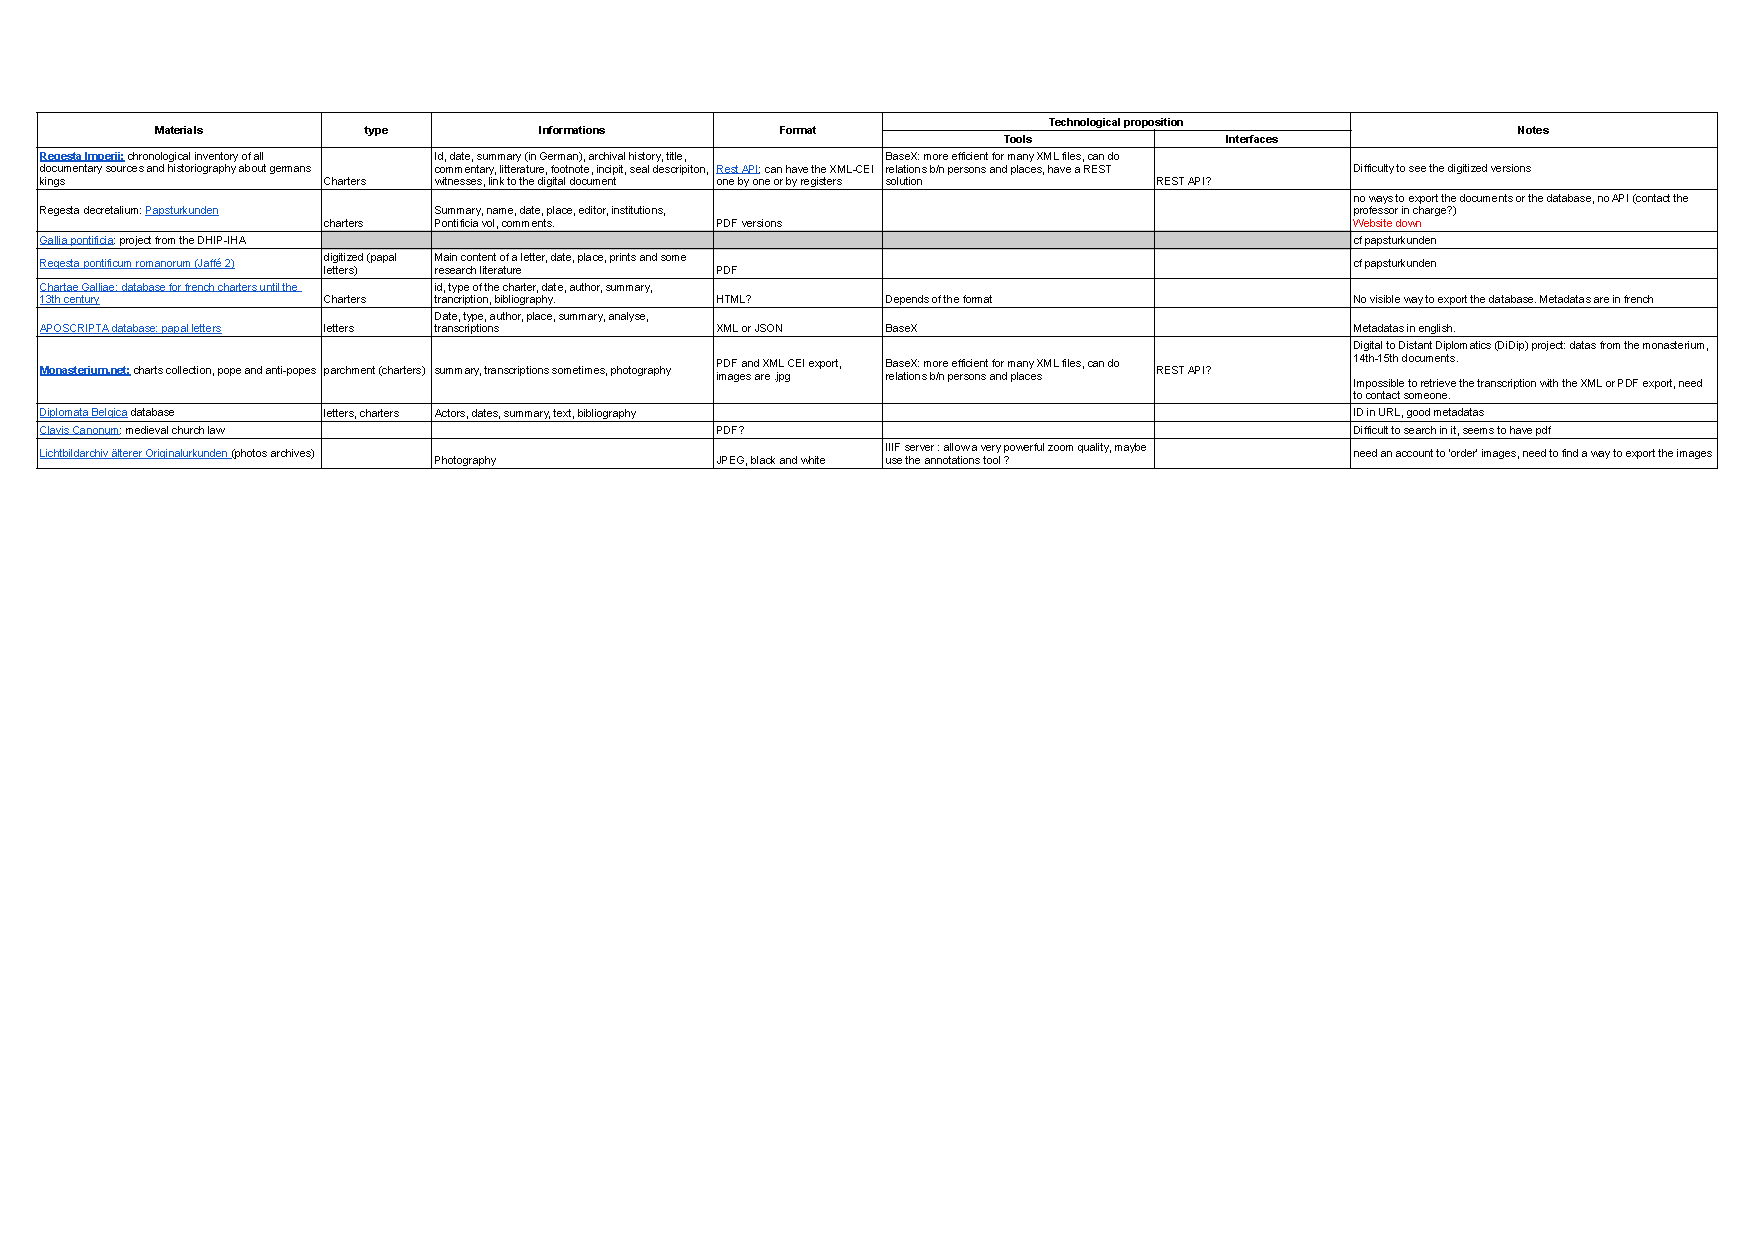
\includepdf[landscape=true]{Templates/Annexes/Corpus_ressources.pdf}
            \end{landscape}

        \chapter[Schéma XML CEI]{Exemple d'un fichier XML CEI issu du RI Online}
            \label{annexe:CEI_schema}

\lstset{style=mystyle}
\begin{lstlisting}[language=XML]
<?xml version="1.0" encoding="UTF-8"?>

<cei xmlns:xsi="http://www.w3.org/2001/XMLSchema-instance" xsi:noNamespaceSchemaLocation="http://www.cei.lmu.de/schema/cei060122.xsd">
		
	<teiHeader>
		<fileDesc>
			<titleStmt>
				<title>Friedrich I. – RI IV,2,2 n. 669</title>
			</titleStmt>
			<editionStmt>
				<p n="volume">RI IV,2,2 - Friedrich I., 2. Lfg. 1158-1168</p>
				<p n="repository">Regesta Imperii Online: <ref type="external" target="http://www.regesta-imperii.de/cei/004-002-002/sources/1159-02-15_1_0_4_2_2_111_669"></ref></p>
			</editionStmt>
			<publicationStmt>
				<p n="authority">Deutsche Kommission für die Bearbeitung der Regesta Imperii e.V. bei der Akademie der Wissenschaften und der Literatur | Mainz</p>
				<publisher>Akademie der Wissenschaften und der Literatur |Mainz – Digitale Akademie</publisher>
				<availability>
					<p>Bereitgestellt unter einer <ref target="https://creativecommons.org/licenses/by/4.0/">Creative Commons Namensnennung (CC BY 4.0)</ref></p>
					<p>Bei Verwendung müssen Sie den Namen des Urhebers und folgenden Link zum Material angeben: <ref type="external" target="http://www.regesta-imperii.de/cei/004-002-002/sources/1159-02-15_1_0_4_2_2_111_669"></ref></p>
				</availability>
				<date></date>
			</publicationStmt>
			<sourceDesc>
				<bibl>
					<idno n="uri">http://www.regesta-imperii.de/id/1159-02-15_1_0_4_2_2_111_669</idno>
					<idno n="department">004</idno>
					<idno n="volume">002</idno>
					<idno n="issue">002</idno>
				</bibl>
			</sourceDesc>
		</fileDesc>
		<encodingDesc>
			<geoDecl xml:id="WGS" datum="WGS84">World Geodetic System</geoDecl>
		</encodingDesc>
		<revisionDesc>
			<p>
				<date type="creation" n="1339417607" value="2012-06-11"></date>
				<date type="lastmod" n="1426241847" value="2015-03-13"></date>
			</p>
		</revisionDesc>
	</teiHeader>

	<charter>
		<chDesc>
			<head>
				<idno>RI IV,2,2 n. 669</idno>
				<issued>
					<issueDate>
						<p>
							<dateRange from="1159-02-15" to="1159-02-15">1159 Februar 15</dateRange>
						</p>
					</issueDate>
					<issuePlace>
						<placeName key="Marengo">Marengo</placeName>
						<location><geo decls="#WGS">44.9167, 8.6667</geo></location>
					</issuePlace>
					<dateOrig>(XV<hi rend="sup">o</hi>  kal. marcii, aput Marengam)</dateOrig>
				</issued>
			</head>
			<relevantPersonal>
					<issuer><persName>Friedrich I.</persName></issuer>
					<recipient><hi rend="spaced">Stadt Asti</hi></recipient>
					<notarius function="chancellor"><hi rend="italic">Reinaldus sacri palacii imperialis canz.</hi></notarius>
					<scribe>verfaßt und geschrieben von RG</scribe>
					<testis function="witnesses">Pfalzgraf Otto (von Wittelsbach), Graf Rudolf von Pfullendorf, Markgraf Obizo Malaspina, Bischof Eberhard von Bamberg und Pfalzgraf Konrad bei Rhein</testis>
			</relevantPersonal>
			<abstract><p>Friedrich nimmt die <span sameAs="recipient"><hi rend="spaced">Stadt Asti</hi> </span>  unter die Herrschaft des Reiches, verleiht den von ihm dort nach freiem Ermessen eingesetzten Rektoren Carioth, Robaldus Gardinus und Petrus Cortessius die namentlich angeführten Regalien (<hi rend="italic">Hec itaque regalia esse dicuntur: moneta, vie publice, aquatica, flumina publica, molandina, furni, forestica, mensure, bancatica, ripatica, portus, argentarie, pedagia, piscationis redditus, sestaria vini et frumenti et eorum, que venduntur ad mensuram, placita, batalia, rubi, restituciones in integrum minorum et alia omnia, que ad regalia iura pertinent</hi>.) in der Stadt, dem Bistum und der Grafschaft mit den genannten Orten vorbehaltlich des königlichen Fodrums gegen einen jährlich an St. Martin (11. November) zu entrichtenden Zins von 150 Mark Silber sowie die Reichsburg Annone mit allen Zugehörungen gegen einen Jahreszins von 50 Mark Silber und sagt zu, die genannten Verleihungen künftig nur den nach seinem Willen aus der Stadt zu erwählenden Amtsträgern zu gewähren. <span n="witnesses">Z.: Pfalzgraf Otto (von Wittelsbach), Graf Rudolf von Pfullendorf, Markgraf Obizo Malaspina, Bischof Eberhard von Bamberg und Pfalzgraf Konrad bei Rhein</span>. - <span n="chancellor"><hi rend="italic">Reinaldus sacri palacii imperialis canz.</hi> </span>; <span n="clerk">verfaßt und geschrieben von RG</span>. <span n="incipit"><hi rend="italic">Universorum Christi et imperii</hi> </span>.</p></abstract>
			<diplomaticAnalysis>
				<div type="incipit"><p><hi rend="italic">Universorum Christi et imperii</hi></p></div>
				<div type="transmission"><p>Kop.: Verstümmelte Abschrift des 14. Jh. im Cod. Astensis f. 4, Stadtarchiv Asti (C); notarielle Abschrift von 1356, Staatsarchiv Turin (D); Abschrift des 17. Jh., Benefizi di qua dai Monti, Miscell. 2 f. 307 ebenda (E). Drucke: Sella, Cod. Astensis 2, 73 n<hi rend="sup">o</hi>  6; MG. DF. I. 259. Reg.: Stumpf 3844.</p></div>
				<div type="commentary"><p>Möglicherweise beriefen sich die Bürger von Asti auf die Zusage weiterer Gunsterweise für den Fall des Italienzuges im DK. III. 60, vgl. die Vorbemerkung zum D. Markgraf Wilhelm von Montferrat (zu seiner früheren Haltung gegenüber Asti vgl. oben Reg. <ref target="http://www.regesta-imperii.de/regesten/4-2-1-friedrich-i/nr/1155-02-01_1_0_4_2_1_274_274.html" type="internal" n="regesten">274</ref>) dürfte sich jedenfalls beim Kaiser zugunsten der Stadt verwendet haben, vgl. Brader, Bonifaz von Montferrat (Hist. Studien 55, 1907) 12 f. - Aus ebendieser Zeit - wohl schon von 1158 - ist ein Treueid der Astenser Bürger für Kaiser Friedrich I. überliefert, Schneider, Neue Dokumente, QFIAB 16 (1914) 24 n<hi rend="sup">o</hi>  5. - Zum D. vgl. auch Opll, Stadt und Reich, 199. - Wohl um eine Verwechslung mit den Ereignissen von 1155 (Reg. <ref target="http://www.regesta-imperii.de/regesten/4-2-1-friedrich-i/nr/1155-02-01_1_0_4_2_1_274_274.html" type="internal" n="regesten">274</ref>) handelt es sich bei dem Bericht des Burchard von Ursberg, ed. Holder-Egger, MG. SS rer. Germ. in us. schol., 32 über eine Einnahme von Asti und Eroberung von Annone um diese Zeit.</p></div>
			</diplomaticAnalysis>
			<div type="resources">
				<list><item><ref target="http://regesta-imperii.digitale-sammlungen.de/seite/ri04_opl1991_0047" type="external" n="bsb">Digitalisat der Buchseite</ref></item><item><ref target="http://www.mgh.de/dmgh/diplomata/resolving/D_F_I_259" type="external" n="unkown">Druck in den MGH Diplomata</ref></item></list>
			</div>
		</chDesc>
	</charter>
</cei>
		

\end{lstlisting}
        
	\chapter[Extraction des lieux]{Script python pour extraire les lieux et leur géolocalisation des fichiers XML}
            \lstset{style=mystyle}
\begin{lstlisting}[language=Python]

import xml.etree.ElementTree as ET
import glob
from pathlib import Path
import csv
from collections import defaultdict

directory = '/home/marine/Documents/RIV_Friedrich1_1122-1190/RIV_Friedrich1_1172-1185'

with open('1172-1185_places.csv', 'w', newline='') as f:
    
    writer = csv.writer(f)

    headers = ['date_start', 'date_end', 'place', 'latitude', 'longitude']

    writer.writerow(headers)

    xml_files_list = list(map(str,Path(directory).glob('**/*.xml')))
    for xml_file in xml_files_list:
        tree = ET.parse(xml_file)
        root = tree.getroot()

        data_list=[]
        issued_tag = root.find('.//issued')

        if issued_tag is not None:
            date = issued_tag.find('.//dateRange')
            place = issued_tag.find('.//placeName')
            coordinate = issued_tag.find('.//geo')
            if place is not None:
                data_list.insert(2, place.text)
                if date is not None:
                    date_from = date.get('from')
                    date_to = date.get('to')
                    data_list.insert(0, date_from)
                    data_list.insert(1, date_to)
                if coordinate is not None:
                    txt= coordinate.text
                    x = txt.split(',')
                    data_list.insert(3, x[0])
                    data_list.insert(4, x[1])

\end{lstlisting}

        \chapter{Statistiques concernant l'utilisation du langage Ruby}
            \section{\href{https://survey.stackoverflow.co/2023/}{Enquêtes Stackoverflow 2023}}
\label{annexe:Ruby_stats}

\subsection{Langages utilisés par les sondé.e.s cette année et ceux envisagés pour l'année suivante}

\begin{quote}
    Quels langages de programmation, de script et de balisage avez-vous utilisés de manière extensive au cours de la dernière année, et lesquels souhaitez-vous utiliser au cours de l'année à venir ? (Si vous avez à la fois travaillé avec le langage et que vous souhaitez continuer à le faire, veuillez cocher les deux cases dans cette ligne.)\footnote{\textit{Which programming, scripting, and markup languages have you done extensive development work in over the past year, and which do you want to work in over the next year? (If you both worked with the language and want to continue to do so, please check both boxes in that row.)}}
\end{quote}


    \begin{figure}[H]
    %centrer l'image
        \centering
        %commande qui permet de charger une image
        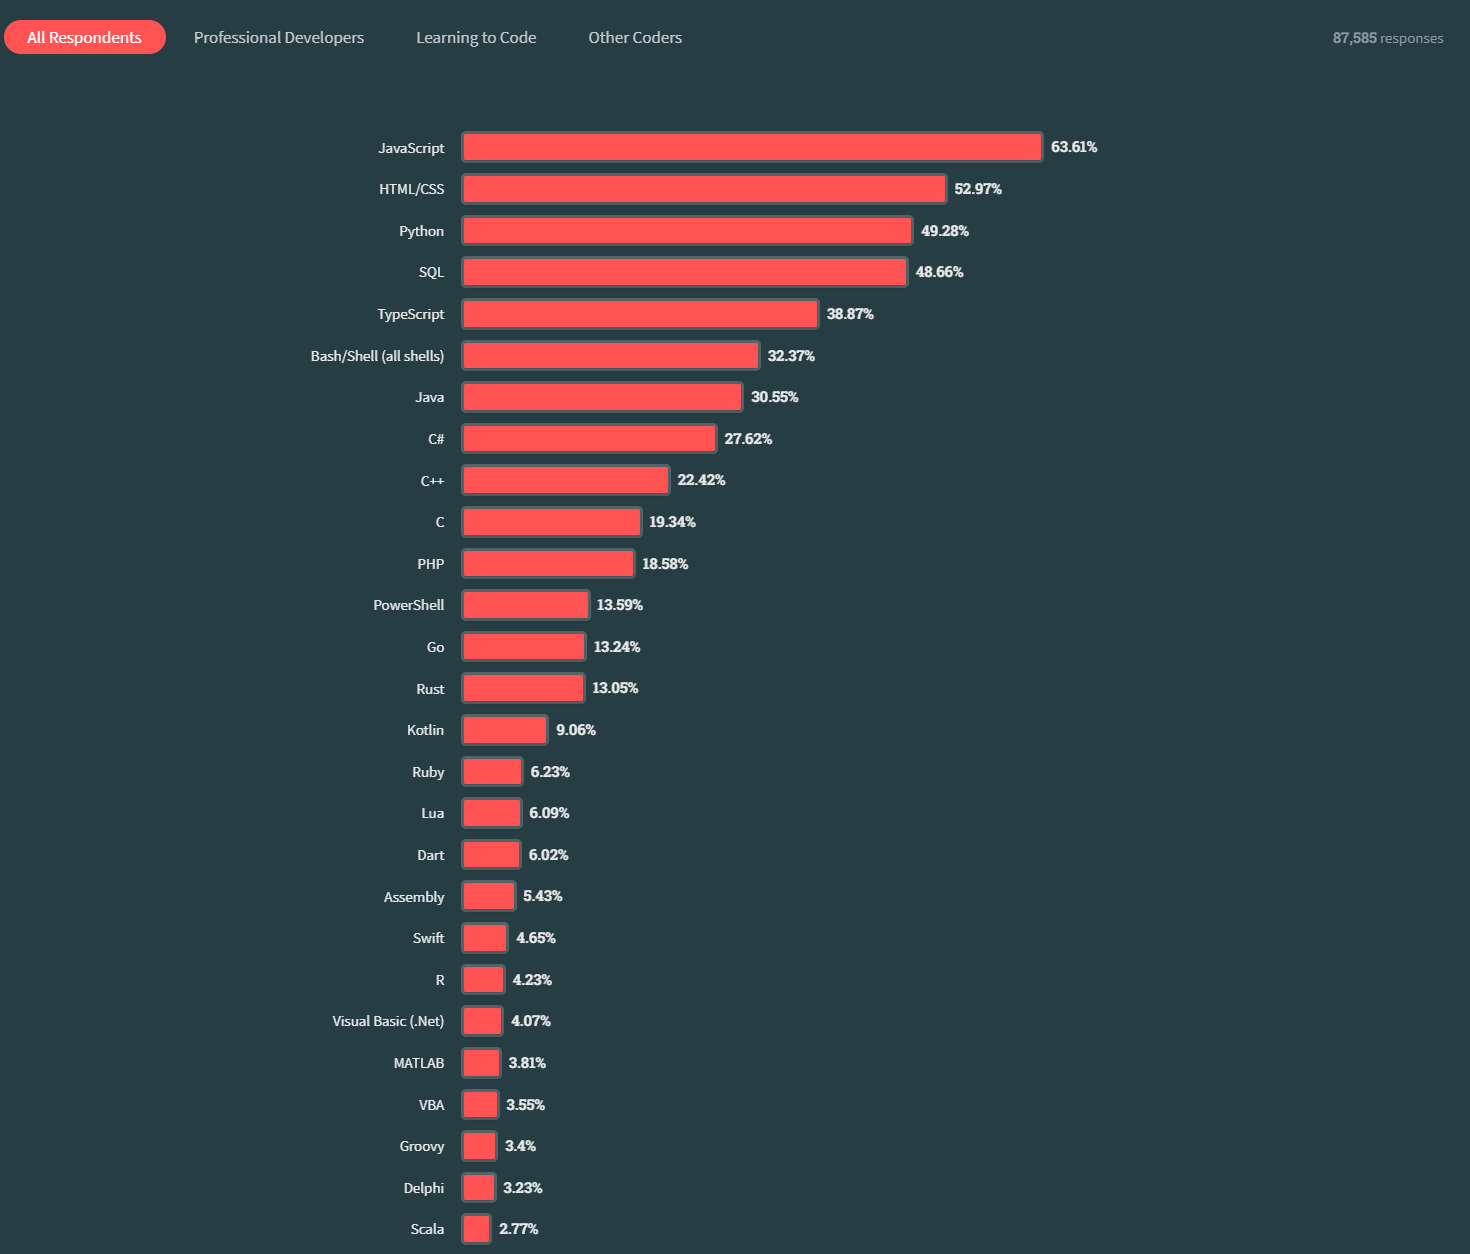
\includegraphics[width=15cm]{images/extrait_sondage_stackoverflow_languages.PNG}
        %légende
        \caption{Capture d'écran d'un diagramme représentant le pourcentage des réponses par langages}
        %label
        \label{fig:StackoverflowLanguages}
    \end{figure}

\subsection{Frameworks utilisés par les sondé.e.s cette année et ceux envisagés pour l'année suivante}

\begin{quote}
    Sur quels \textit{framework} et quelles technologies web avez-vous effectué un travail de développement important au cours de la dernière année, et lesquels souhaitez-vous utiliser au cours de l'année à venir ? (Si vous avez à la fois travaillé avec le cadre et que vous souhaitez continuer à le faire, veuillez cocher les deux cases dans cette ligne.)\footnote{\textit{Which web frameworks and web technologies have you done extensive development work in over the past year, and which do you want to work in over the next year? (If you both worked with the framework and want to continue to do so, please check both boxes in that row.)}}
\end{quote}

\begin{figure}[H]
    %centrer l'image
        \centering
        %commande qui permet de charger une image
        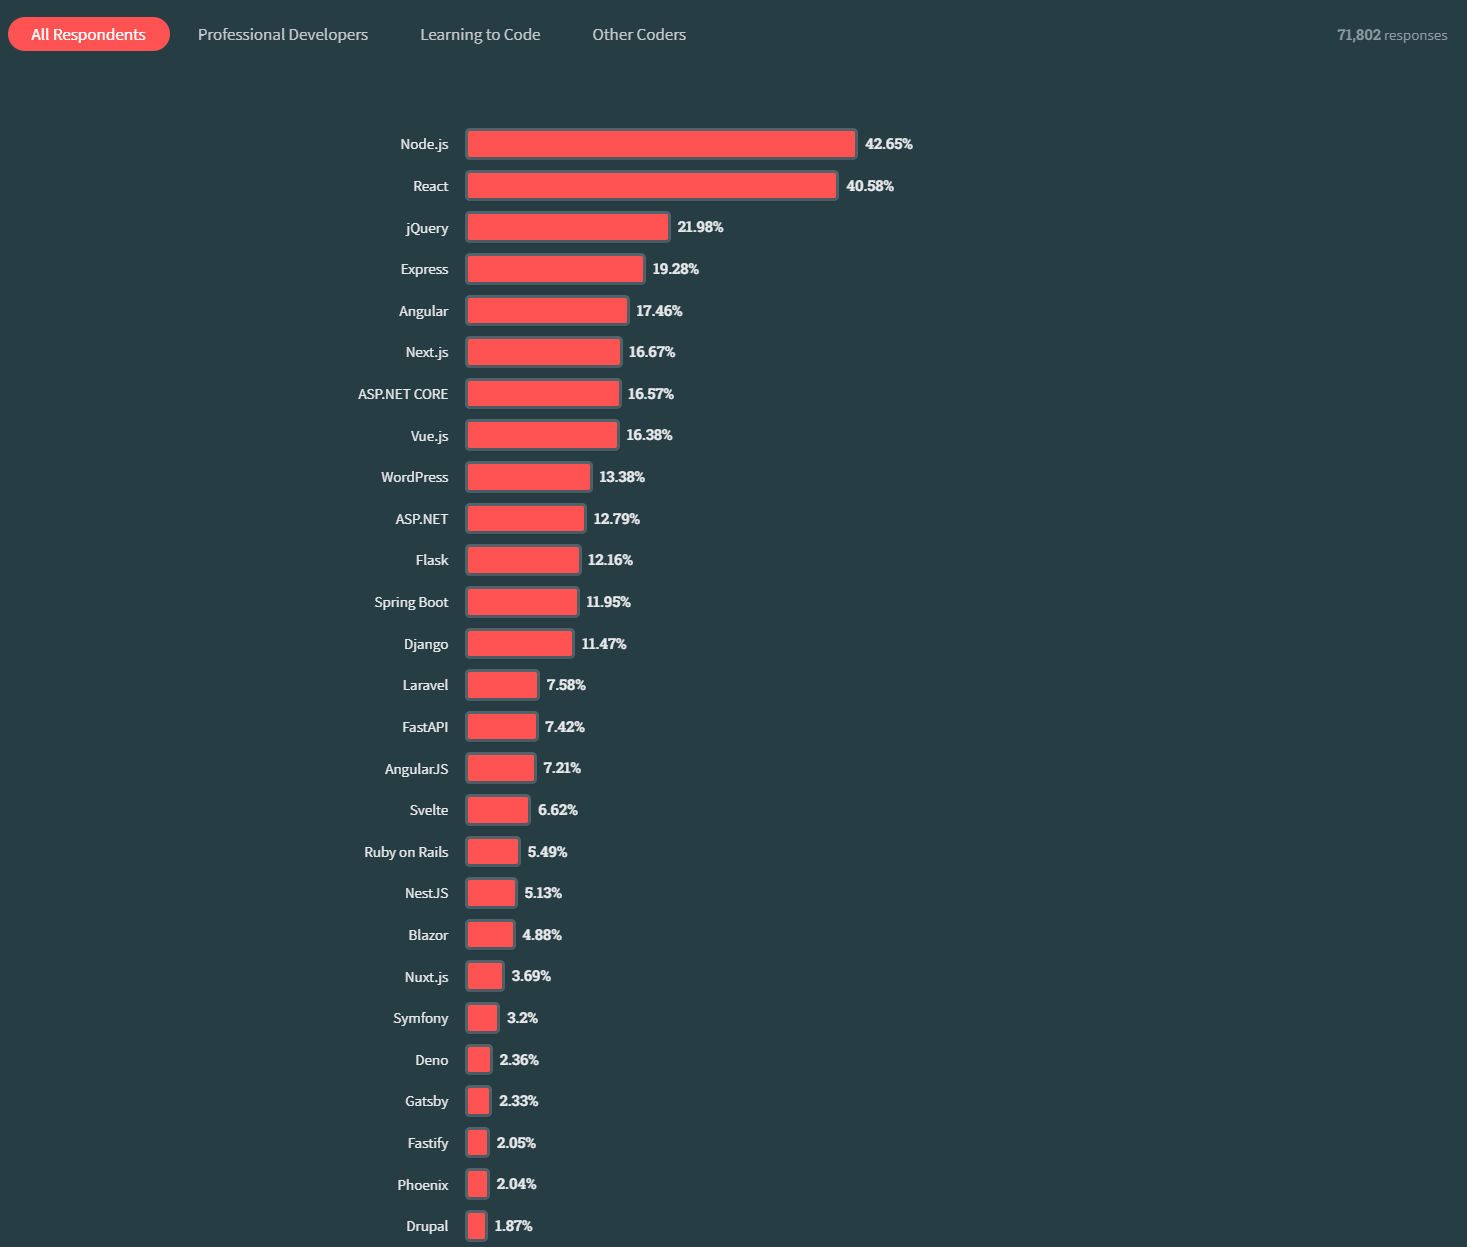
\includegraphics[width=15cm]{images/extrait_sondage_stackoverflow_framework.PNG}
        %légende
        \caption{Capture d'écran d'un diagramme représentant le pourcentage des réponses par frameworks}
        %label
        \label{fig:StackoverflowFrameworks}
\end{figure}


\section{Évolution de l'utilisation du langage Ruby}

\begin{figure}[H]
    %centrer l'image
        \centering
        %commande qui permet de charger une image
        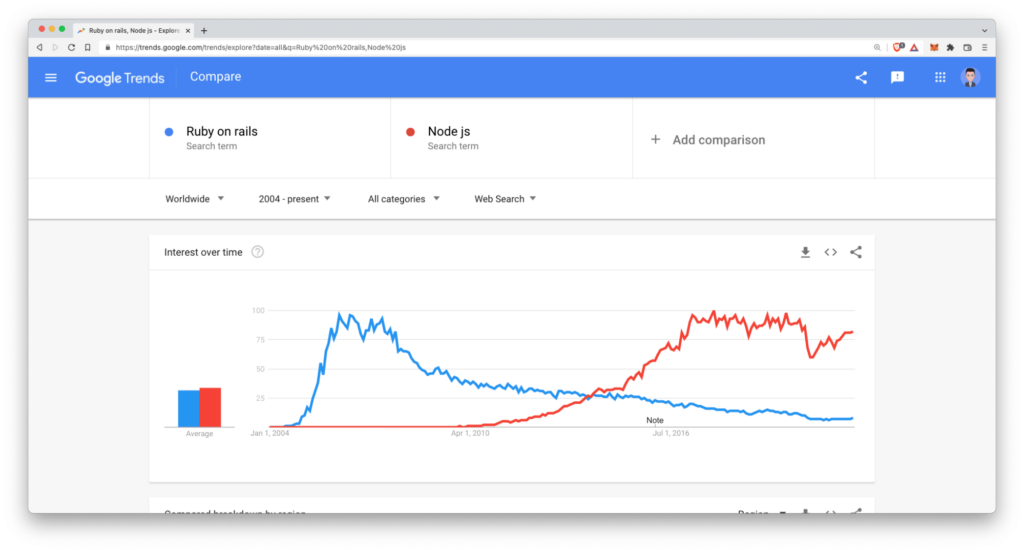
\includegraphics[width=15cm]{images/google-trends-ruby-vs-node.png}
        %légende
        \caption{Capture d'écran comparaison de l'intérêt pour Ruby et pour Node js entre 2004 à aujourd'hui sur Google Trends}
        %label
        \label{fig:RubyvsNodejs}
\end{figure}

\begin{figure}[H]
    %centrer l'image
        \centering
        %commande qui permet de charger une image
        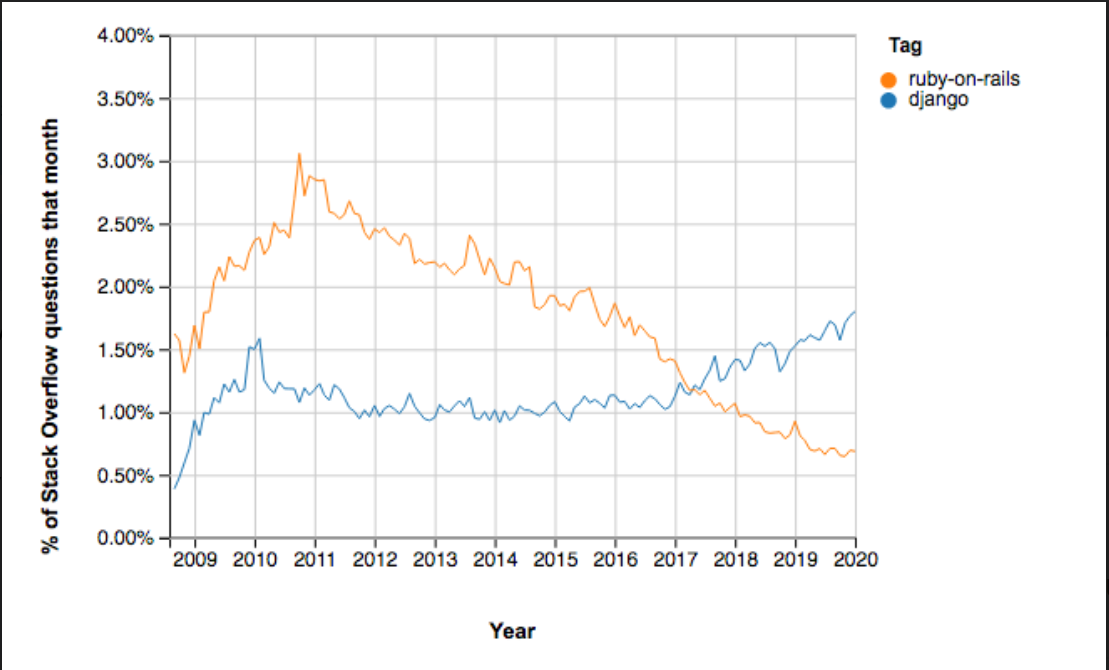
\includegraphics[width=15cm]{images/Ruby_vs_Django_trend.png}
        %légende
        \caption{Capture d'écran comparaison de l'intérêt pour Ruby et pour Django entre 2004 à 2020 sur Google Trends}
        %label
        \label{fig:RubyvsDjango}
\end{figure}



	
	\backmatter


% si figures
 \listoffigures

% si tables
%	\listoftables

	\tableofcontents
	
\end{document}